% =====================================================================
%  Draw-to-Web — Graduation Project Report
%  LaTeX scaffold. Compile with:  latexmk -pdf main.tex
%  (uses biblatex + biber; Overleaf handles this automatically)
%
%  HOW THIS SCAFFOLD WORKS
%  - Each numbered chapter lives in sections/NN-*.tex and is \input below.
%  - Every chapter file starts with a "% SOURCES:" comment block listing the
%    repo files that back it, so you write from evidence, not memory.
%  - Content marked  % TODO  is yours to write/verify.
%  - Content already drafted from the repo docs is real but should be reviewed.
%  - DO NOT invent the pending perf numbers (render-layer FPS / rehearsal) —
%    they are tracked in issue #95 and marked as such in ch. 10–11.
% =====================================================================
\documentclass[12pt,a4paper,oneside]{report}

% ---- Encoding & fonts (pdfLaTeX) ----
\usepackage[T1]{fontenc}
\usepackage[utf8]{inputenc}
\usepackage{lmodern}
\usepackage{amssymb} % \checkmark and math symbols used in tables

% ---- Layout ----
\usepackage[a4paper,margin=2.5cm,headheight=15pt]{geometry}
\usepackage{setspace}
\onehalfspacing
\usepackage{parskip}
\usepackage{emptypage}

% ---- Graphics & figures ----
\usepackage{graphicx}
\graphicspath{{figures/}}
\usepackage{caption}
\usepackage{float}

% ---- Diagrams (native TikZ UML — no external renderer needed) ----
% The three UML diagrams (class / use-case / sequence) in ch. 7 are drawn
% directly in TikZ so the report is self-contained: it compiles on Overleaf
% or any TeX Live / MiKTeX install with no PlantUML, Mermaid, Java or dot.
\usepackage{tikz}
\usetikzlibrary{positioning, arrows.meta, shapes.multipart, shapes.geometric,
  fit, calc, backgrounds}
\tikzset{
  % --- UML class boxes (name compartment | attributes compartment) ---
  umlclass/.style={
    draw, rectangle split, rectangle split parts=2, fill=blue!6,
    font=\ttfamily\scriptsize, text width=33mm, align=left,
    inner sep=3pt, line width=0.4pt, rounded corners=1pt,
  },
  umlabstract/.style={umlclass, fill=violet!8},
  umlvalue/.style={umlclass, fill=teal!7, text width=30mm},
  umlnode/.style={umlclass, fill=orange!8, text width=27mm},
  % --- UML relations ---
  inherit/.style={-{Triangle[open, length=3.4mm, width=3.4mm]}, line width=0.5pt},
  compose/.style={{Diamond[fill=black, length=3.2mm, width=2.2mm]}-{Stealth[length=2mm]},
    line width=0.5pt},
  aggregate/.style={{Diamond[open, length=3.2mm, width=2.2mm]}-{Stealth[length=2mm]},
    line width=0.5pt},
  % --- Use-case diagram ---
  usecase/.style={draw, ellipse, align=center, font=\footnotesize,
    minimum width=32mm, minimum height=11mm, fill=blue!5, inner sep=1pt},
  ucedge/.style={line width=0.5pt},
  ucinclude/.style={-{Stealth[length=2.2mm]}, dashed, line width=0.5pt},
  ucactor/.pic={
    \draw[line width=0.5pt] (0,0) circle (2.2mm);
    \draw[line width=0.5pt] (0,-2.2mm) -- (0,-9mm);
    \draw[line width=0.5pt] (-4mm,-5mm) -- (4mm,-5mm);
    \draw[line width=0.5pt] (0,-9mm) -- (-3.6mm,-14mm);
    \draw[line width=0.5pt] (0,-9mm) -- (3.6mm,-14mm);
  },
  % --- Sequence diagram ---
  seqbox/.style={draw, fill=blue!8, minimum width=24mm, minimum height=7mm,
    font=\small, align=center, rounded corners=1pt},
  lifeline/.style={dashed, line width=0.4pt, gray},
  activation/.style={draw, fill=blue!12, minimum width=2.4mm},
  seqmsg/.style={-{Stealth[length=2.4mm]}, line width=0.5pt},
  seqret/.style={-{Stealth[length=2.4mm]}, line width=0.5pt, dashed},
}

% ---- Tables ----
\usepackage{booktabs}
\usepackage{tabularx}
\usepackage{array}
\usepackage{longtable}

% ---- Code listings ----
\usepackage{xcolor}
\usepackage{listings}
\definecolor{codebg}{RGB}{247,247,247}
\definecolor{codekw}{RGB}{0,92,197}
\definecolor{codecm}{RGB}{106,115,125}
\definecolor{codestr}{RGB}{3,47,98}
\lstset{
  basicstyle=\ttfamily\footnotesize,
  backgroundcolor=\color{codebg},
  keywordstyle=\color{codekw}\bfseries,
  commentstyle=\color{codecm}\itshape,
  stringstyle=\color{codestr},
  numbers=left, numberstyle=\tiny\color{codecm}, numbersep=8pt,
  breaklines=true, showstringspaces=false, frame=single, framerule=0pt,
  captionpos=b, tabsize=2,
}

% ---- Misc ----
\usepackage{enumitem}
\usepackage{csquotes}
\usepackage{fancyhdr}
\pagestyle{fancy}
\fancyhf{}
\fancyhead[L]{\nouppercase{\leftmark}}
\fancyhead[R]{\thepage}
\renewcommand{\headrulewidth}{0.4pt}

% ---- Bibliography (biblatex + biber, IEEE-like numeric) ----
\usepackage[backend=biber,style=numeric-comp,sorting=none]{biblatex}
\addbibresource{references.bib}

% ---- Hyperlinks (load near-last) ----
\usepackage[hidelinks,breaklinks]{hyperref}
\hypersetup{
  pdftitle={Draw-to-Web: A Desktop Visual Authoring Tool for Semantic, Responsive Web Pages},
  pdfauthor={Ibrahim Haski},
  bookmarksnumbered=true,
}

% =====================================================================
\begin{document}

% ------------------------- TITLE PAGE -------------------------
% NOTE: A few identity details cannot be derived from the repository and are
% left as clearly-marked placeholders in [brackets] — replace them with your
% own values: the faculty/department (if different), the supervisor's name,
% and the third author's student ID. Add the university logo where indicated.
\begin{titlepage}
  \centering
  % \includegraphics[width=3cm]{university-logo.png}\\[0.4cm]  % add logo here
  {\Large \textbf{Antioch University}}\\[0.3cm]
  {\large Faculty of Informatics Engineering --- Department of Software Engineering}\\[2.5cm]

  \rule{\linewidth}{0.4mm}\\[0.6cm]
  {\huge \bfseries Draw-to-Web}\\[0.3cm]
  {\Large A Desktop Visual Authoring Tool for Generating\\[0.2cm]
   Semantic, Responsive, Accessible Web Pages}\\[0.4cm]
  % Arabic title: add here if your programme requires it (needs a UTF-8 Arabic
  % font, e.g. compile with XeLaTeX + polyglossia, or paste as an image).
  % {\large \itshape [العنوان بالعربية]}\\[0.4cm]
  \rule{\linewidth}{0.4mm}\\[1.5cm]

  \begin{minipage}{0.45\textwidth}
    \begin{flushleft}\large
      \textit{Prepared by:}\\
      Ibrahim Haski \quad (221116)\\
      Yousef Deeb \quad (112004)\\
      Abd Alrazak Qahwaji \quad ([ID])\\
    \end{flushleft}
  \end{minipage}
  \hfill
  \begin{minipage}{0.45\textwidth}
    \begin{flushright}\large
      \textit{Supervised by:}\\
      \textrm{[Supervisor Name]}\\
    \end{flushright}
  \end{minipage}\\[3cm]

  {\large \textbf{Graduation Project Report}}\\[0.3cm]
  {\large Academic Year 2025--2026}\\[0.5cm]
  \vfill
\end{titlepage}

% ------------------------- FRONT MATTER -------------------------
\pagenumbering{roman}

% TODO (optional): Abstract, Acknowledgements, Dedication
\chapter*{Abstract}
\addcontentsline{toc}{chapter}{Abstract}
% SOURCES: README.md (intro), docs/1.0.0v/supervisor-report.md (§1, §13),
%          draft/Features/features.md
% GUIDANCE: 150–250 words — problem, approach, what was built, key results.
% TODO: write the abstract last, once ch. 11 (Results) is final.
% SOURCES: README.md; docs/1.0.0v/supervisor-report.md (§1, §13); draft/Features/features.md
% Abstract — written last, from the verified results in ch. 11. The pending
% render-layer performance figures (issue #95) are deliberately NOT claimed here.

Authoring a web page that is at once \emph{semantic}, \emph{responsive}, and
\emph{accessible} still demands specialist skill, and the visual ``no-code''
builders that promise to remove that barrier typically do so at the expense of
output quality: heavy proprietary runtimes, non-semantic markup, absolute
positioning, and pages that are difficult to audit for accessibility.
\textbf{Draw-to-Web} is a desktop application that resolves this tension. A single
\emph{Document Model} is the only source of truth: the canvas is a rendering of
that model, and a deterministic generator walks the same model to emit semantic
HTML5, tokens-driven CSS, and opt-in, independently toggleable JavaScript. When no
runtime behaviour is enabled, the output contains no \texttt{<script>} at all.
Accessibility is enforced as a build-time hard gate --- \texttt{axe-core} runs on
the generated HTML and blocks export on any \emph{critical} or \emph{serious}
violation --- rather than left to manual review. The system was built as a
strict-TypeScript Electron + React application with a Zustand/immer state layer, a
Zod-validated process boundary, and a nine-stage export pipeline. Version~1.0.0
adds three authoring surfaces that reuse the same operations and export path:
\emph{draw-to-create} (draw a rectangle to place an element), \emph{match-layout}
(adopt a professional design from a rough draft), and a headless \emph{Model
Context Protocol} (MCP) server. The v1.0.0 release is green across all automated
gates: \textbf{1042 automated tests} across 110 files pass, linting and strict
type-checking are clean, the accessibility gate is enforced on every export path,
and the data-layer and export performance budgets are met with wide margins (for
example a full nine-stage export of a portfolio page completes in roughly
0.2--0.3~s against a 10~s budget). The work shows that visual, no-code authoring
and hand-written-quality output need not be opposites.

\vspace{0.6em}
\noindent\textbf{Keywords:} visual web authoring; no-code; semantic HTML5;
web accessibility (WCAG); design tokens; deterministic code generation; Electron;
Model Context Protocol.


\tableofcontents
\listoffigures
\listoftables

% ------------------------- BODY -------------------------
\clearpage
\pagenumbering{arabic}

% SOURCES: README.md; draft/Features/features.md; docs/0.2.0v/plan.md (§1 North Star,
%          §2 Scope Tiers); docs/1.0.0v/supervisor-report.md (§1)

\chapter{Introduction}
\label{ch:introduction}

\section{Field of Work}
The modern web is built from three languages --- HTML for structure, CSS for
presentation, and JavaScript for behaviour --- yet authoring a page that is
simultaneously \emph{semantic}, \emph{responsive}, and \emph{accessible} remains a
specialised skill. Over the last decade a class of \emph{visual web builders} ---
tools such as Webflow, Framer, and Wix --- has lowered the barrier to entry by
letting users compose pages on a canvas rather than in a text editor
\cite{webflow,framer,wix}. These tools trade code for direct manipulation, which
is a genuine advance in accessibility of \emph{authoring}; but they frequently do
so at the cost of the \emph{output}: heavy client-side runtimes, non-semantic
``div soup'', absolute positioning that breaks on unexpected viewports, and markup
that is difficult to audit against accessibility standards.

Two forces sharpen the problem. First, the \emph{no-code / low-code} movement has
brought a large, non-technical audience to web authoring, so the quality of what a
builder emits is now the quality that most sites inherit. Second, accessibility
has moved from a courtesy to a requirement: the Web Content Accessibility
Guidelines (WCAG) \cite{wcag21} are referenced by legislation in many
jurisdictions, and semantic HTML \cite{whatwg-html} is the foundation on which
assistive technology depends. In parallel, professional front-end practice has
converged on \emph{design tokens} --- named, themeable primitives for colour,
spacing, and typography --- as the disciplined way to keep a design system
consistent. A tool built today should treat semantics, accessibility, and tokens
as first-class concerns rather than as afterthoughts to be patched on later.

\section{Problem Statement}
The core tension this project addresses is that \emph{visual authoring} and
\emph{high-quality output} are usually treated as opposites. A user who cannot
write code is typically forced to accept whatever markup a builder emits, with no
guarantee of semantic structure, accessibility compliance, or portability, and
often with a hard dependency on the vendor's hosting and runtime. The question the
project sets out to answer is therefore concrete and testable:

\begin{quote}
\itshape Can a canvas-based visual editor produce hand-written-quality output ---
semantic, deterministic, accessibility-gated HTML and CSS with only opt-in
JavaScript --- without requiring the author to write or read code, and without
locking the result to a proprietary platform?
\end{quote}

\section{Proposed Solution}
Draw-to-Web is a desktop application that answers this question by making a single
\emph{Document Model} the only source of truth. The canvas is a rendering of that
model; a deterministic generator walks the same model to emit semantic HTML5,
tokens-driven CSS, and opt-in vetted JavaScript. Every visual property is
token-bindable and per-breakpoint, so theming and responsiveness fall out of the
data model rather than being bolted on. Accessibility is enforced by a hard gate
(\texttt{axe-core}) that blocks export on any critical or serious violation, and
the output is formatted with \texttt{prettier} so that it reads as though a human
wrote it. Because the tool is a local desktop application, the exported bundle is a
plain folder of files with no build step and no mandatory runtime --- fully
portable, with no vendor lock-in.

Version~1.0.0 extends this foundation with three authoring surfaces that make the
tool faster to use without weakening any of its guarantees, because each reuses the
same document operations and export pipeline: \emph{draw-to-create} (draw a
rectangle and the system proposes the element to place), \emph{match-layout}
(sketch a rough structure and adopt a bundled professional design that matches it),
and a headless \emph{Model Context Protocol} (MCP) server that drives the whole
pipeline programmatically \cite{mcp-spec}, so the builder can be scripted by an
agent or a client with no graphical interface.

\section{Report Organisation}
The remainder of this report is organised as follows. Chapter~\ref{ch:objective}
states the primary and specific objectives and the project scope.
Chapter~\ref{ch:methodology} describes the work methodology: the task-driven,
milestone-gated process, the ownership model, and the quality gates.
Chapter~\ref{ch:plan} presents the implementation plan and the deviations from it.
Chapter~\ref{ch:requirements} gathers the functional and non-functional
requirements and the primary use cases. Chapter~\ref{ch:refstudy} reviews similar
projects and positions Draw-to-Web against them. Chapter~\ref{ch:analysis} gives
the system analysis, including the UML class, use-case, and sequence diagrams.
Chapter~\ref{ch:tech} lists the technologies used and justifies each choice.
Chapter~\ref{ch:impl} details the implementation. Chapter~\ref{ch:testing} covers
testing and evaluation against the defined budgets, and Chapter~\ref{ch:results}
reports the results against the objectives, states the limitations honestly, and
concludes.

% SOURCES: docs/0.2.0v/plan.md (§1 North Star, §4 Guiding Principles);
%          README.md (Key invariants); CLAUDE.md (Core Design Rules)

\chapter{Project Objective}
\label{ch:objective}

\section{Primary Objective}
The primary objective is to design and build a desktop application that lets
non-developers author modern, semantic, responsive, and accessible web pages by
direct manipulation on a canvas, and that exports a portable, human-readable
HTML/CSS bundle with opt-in, independently toggleable JavaScript behaviours. The
guiding principle throughout is that \emph{output quality is a first-class
requirement}: the tool must never force the author to choose between the
convenience of visual editing and the quality of the result.

\section{Specific Objectives}
The primary objective decomposes into six specific, measurable sub-objectives.
Each is written so that Chapters~\ref{ch:testing} and~\ref{ch:results} can report
on it directly.

\begin{enumerate}[label=\textbf{O\arabic*.}, leftmargin=3.2em]
  \item \textbf{Single source of truth.} Represent every page as one Document
        Model. The canvas renders it and the generator walks it; no component owns
        page state independently. \emph{Measurable by:} a one-directional data-flow
        architecture in which the store is the only mutable state.
  \item \textbf{Semantic, deterministic output.} Emit semantic HTML5 chosen by
        role (\texttt{<header>}, \texttt{<nav>}, \texttt{<main>},
        \texttt{<section>}, \texttt{<article>}, \texttt{<footer>}, \texttt{<button>},
        \texttt{<a>}) and guarantee byte-identical output for identical input ---
        no timestamps and no random identifiers. \emph{Measurable by:} a
        determinism test and a no-\texttt{position:absolute} invariant test.
  \item \textbf{Accessibility by construction.} Enforce a hard gate that blocks
        export on any critical or serious accessibility violation, and honour a
        single \texttt{<h1>}, unbroken heading order, \texttt{alt} text on every
        image, ARIA labels on icon-only controls, visible focus indicators, and
        the \texttt{prefers-reduced-motion} preference. \emph{Measurable by:} the
        \texttt{axe-core} gate and the validation rule suite.
  \item \textbf{Tokens-driven, responsive styling.} Drive all styling through
        design tokens with light/dark theming and per-breakpoint values
        (desktop, tablet, mobile, small). \emph{Measurable by:} \texttt{var()}
        references in output, a \texttt{:root} token block, and emitted media
        queries.
  \item \textbf{Opt-in, vetted runtime.} Ship only the JavaScript the author
        enables; with all behaviours disabled, produce JavaScript-free output.
        \emph{Measurable by:} the all-flags-off ``no \texttt{<script>}'' test.
  \item \textbf{Accessible authoring surfaces (v1.0.0).} Provide draw-to-create,
        match-layout, and a headless MCP server, each reusing the same document
        operations and export pipeline so they inherit the same guarantees.
        \emph{Measurable by:} their dedicated test suites and the fact that
        headless exports pass the same accessibility gate.
\end{enumerate}

\section{Scope}
% SOURCES: docs/0.2.0v/plan.md (§2 Scope Tiers, §22 Out of Scope); draft/Features/*.md
The project deliberately bounds its scope into three tiers. \textbf{Tier~1} --- the
target output-capability set specified in \texttt{draft/Features/features.md} --- is
fully in scope and is what the builder must be able to \emph{produce}: semantic,
tokens-driven, accessible, responsive pages with opt-in runtime behaviour.
\textbf{Tier~2} is the broader editor-experience ``nice to have'' set, and
\textbf{Tier~3} is the long-horizon product concern (cloud, accounts, billing, and
real-time collaboration); both are out of scope for this sprint. The one conscious
exception is that three Tier~2 authoring surfaces --- draw-to-create,
match-layout, and the MCP server --- were brought forward into v1.0.0 because they
proved to be the most demonstrable capabilities in the product and, crucially,
because their cores are pure and headless and reuse the existing operations, so
they added capability without adding architectural risk (this decision, and the
scope-line move it entails, is recorded in the project decision log as D-03 and
discussed in Section~\ref{sec:deviations}).

% SOURCES: docs/0.2.0v/plan.md (§4, §6, §17, §7); CLAUDE.md (Sprint Model, Git Workflow);
%          .claude/rules/*; docs/1.0.0v/supervisor-report.md (§8)

\chapter{Work Methodology}
\label{ch:methodology}

This chapter describes \emph{how} the team worked --- the development model,
ownership structure, interface contracts, and quality gates --- rather than what
was built. The process was unusually well documented for a student project, and
that discipline is itself one of the project's results.

\section{Development Model: Task-Driven Milestones}
Development followed a \emph{task-driven, milestone-gated} model rather than a
fixed time-box. Progress was unlocked by completing the tasks that gate each
milestone, not by the calendar: a milestone was ``done'' only when its gating tasks
were complete \emph{and} every quality gate was green. Five milestones carried the
work from \textbf{M1 (Foundation)} through \textbf{M5 (Polish + Demo)}, followed by
the \textbf{v1.0.0} demo cut (the milestone table is reproduced in
Chapter~\ref{ch:plan}, Table~\ref{tab:milestones}). Every task carried a single
owner, a priority (\texttt{P0} blocks the demo, \texttt{P1} is a Tier-1 feature,
\texttt{P2} is polish), and explicit \texttt{depends:}/\texttt{blocks:} links, so
the critical path was always visible and the Document Model --- which blocks every
other area --- was scheduled to land first.

\section{Team Structure and Ownership}
% SOURCES: CLAUDE.md (Module Ownership); docs/0.2.0v/plan.md (§10 Tasks)
Three engineers owned disjoint areas of the codebase, which kept merge contention
low and made every file traceable to a responsible owner:

\begin{itemize}[leftmargin=1.5em]
  \item \textbf{Ibrahim Haski} --- the Document Model
        (\texttt{types}, \texttt{schemas}, \texttt{operations}, \texttt{tokens},
        \texttt{validation}, \texttt{migrations}, \texttt{presets}), the output
        pipeline (\texttt{generator}, \texttt{runtime}, \texttt{seo},
        \texttt{export}), the Electron shell and IPC, and the build/CI
        configuration.
  \item \textbf{Yousef Deeb} --- the state layer: the Zustand stores, undo/redo
        history implemented as \texttt{immer} patches, persistence
        (the \texttt{.dtw} file format), autosave and crash recovery, and
        external-change reload; and, in v1.0.0, the draw / match / MCP surfaces.
  \item \textbf{Abd Alrazak Qahwaji} --- the user interface: the canvas, the
        properties, layers, and tokens panels, the sidebar, the topbar, and the
        semantic-inference hints the generator consumes.
\end{itemize}

\section{Cross-Owner Contracts}
% SOURCES: docs/0.2.0v/plan.md (§6 Contracts C1–C12); docs/0.2.0v/architecture.md (§6)
Because three people worked in parallel against a shared model, the interfaces
between owners were fixed as twelve numbered \emph{contracts} (C1--C12). These
include the shared types (C1), the Zod schemas kept in lockstep with them (C2), the
operation set (C3), the typed IPC surface (C4), the store hooks (C5), the generator
entry point (C6), the presets registry (C7), the validation function (C8), the
token resolver (C9), the semantic-inference hint (C10), the image-upload IPC
contract (C11), and the export orchestrator (C12). Any breaking change to a
contract required a pull request labelled \texttt{contract-change} and a review
from the named downstream consumer; this single rule is what allowed the three
lanes to move quickly without silently diverging.

\section{Quality Gates and Tooling}
% SOURCES: .claude/rules/git.md, preflight.md; CLAUDE.md (Commands, Code Quality)
Every push had to pass three gates: linting (ESLint + Prettier), strict
type-checking (TypeScript in strict mode across the main, preload, and renderer
\texttt{tsconfig}s), and the full automated test suite. These were enforced twice
--- locally by a \texttt{husky} pre-push hook and again in continuous integration
--- so a red build could not reach \texttt{main}. On top of the three gates,
specialised automated review passes checked properties that unit tests do not
naturally cover: output \emph{determinism}, the no-\texttt{position:absolute}
invariant, accessibility of generated output, and correctness of any contract
change. A weekly integration ritual merged all open feature branches, ran the full
matrix, and held a short debrief with no new commits, which caught cross-lane
integration problems early rather than at release. As a matter of academic
integrity, the project also enforced a ``no AI attribution'' policy on all commits,
pull requests, and reviews; the work and its authorship are the students' own.

\section{Version Control and Release Workflow}
% SOURCES: .claude/rules/git.md; .github/workflows/{ci,release}.yml; CHANGELOG.md
Work used \emph{conventional commits} (for example
\texttt{feat(generator): emit skip-to-content link}) on short-lived feature
branches that were squash-merged into \texttt{main}; the \texttt{main} branch was
never force-pushed. Releases were tag-driven: pushing a \texttt{v*} tag triggered a
per-operating-system build matrix that produced native installers (Windows NSIS,
Linux AppImage/deb, macOS dmg/zip) and published a single GitHub Release. Versions
progressed v0.1.0 $\rightarrow$ v0.2.0 $\rightarrow$ v0.3.0 $\rightarrow$
\textbf{v1.0.0}, with each tag corresponding to a completed milestone.

% SOURCES: docs/0.2.0v/plan.md (§10 Tasks, §17 Milestones, §9 Library-to-Feature Map);
%          docs/CHANGELOG.md; docs/DECISIONS.md; docs/1.0.0v/supervisor-report.md (§1)

\chapter{Project Implementation Plan}
\label{ch:plan}

\section{Milestone Breakdown}
The work was divided into five gated milestones plus the v1.0.0 demo cut
(Table~\ref{tab:milestones}). The ordering encodes the technical dependencies of
the system: the Document Model and the store had to exist before anything could be
rendered or generated (M1); themable output required the token system (M2);
composition and responsiveness required presets and per-breakpoint style (M3); the
runtime, SEO, and the accessibility gate hardened the output (M4); and polish plus
a released artifact completed the sprint (M5). Each milestone was ``done'' only
when its gating tasks were complete and all quality gates were green.

\begin{table}[H]
  \centering
  \caption{Milestone plan and definition of done.}
  \label{tab:milestones}
  \begin{tabularx}{\linewidth}{@{}l l X@{}}
    \toprule
    \textbf{Milestone} & \textbf{Theme} & \textbf{Definition of done (summary)} \\
    \midrule
    M1 & Foundation            & Types + store + recursive canvas + undo/redo + persistence + basic generator + export shell. \\
    M2 & Tokens + Themes       & Token registry + theme toggle + auto-layout + \texttt{:root} block + \texttt{var()} refs. \\
    M3 & Composition + Resp.   & 6+ presets + hover/focus states + breakpoint switcher + multi-select + image upload. \\
    M4 & Runtime + Hardening   & Full runtime snippets + SEO + validation console + \texttt{axe-core} gate + templates. \\
    M5 & Polish + Demo         & Polish + performance budgets + release artifact + rehearsed demo. \\
    v1.0.0 & Demo cut          & draw-to-create + match-layout + headless MCP server; released with native installers. \\
    \bottomrule
  \end{tabularx}
\end{table}

\section{Task Allocation and the Critical Path}
% SOURCES: docs/0.2.0v/plan.md (§10); CLAUDE.md (Module Ownership)
Tasks were identified by owner and area --- for example \texttt{I-DOC-*} for the
Document Model, \texttt{I-GEN-*} for the generator, \texttt{I-RUN-*} for runtime
snippets, \texttt{Y-*} for the store, and \texttt{L-*} for the user interface ---
each with a priority and explicit dependency links. The critical path ran through
the Document Model: because the types (C1), schemas (C2), and operations (C3) are
consumed by every other lane, the \texttt{I-DOC} tasks were front-loaded and had to
land before the store, canvas, and generator could be written against a stable
shape. Table~\ref{tab:allocation} summarises the allocation of areas to owners.

\begin{table}[H]
  \centering
  \caption{Allocation of work areas to owners.}
  \label{tab:allocation}
  \small
  \begin{tabularx}{\linewidth}{@{}l X@{}}
    \toprule
    \textbf{Owner} & \textbf{Areas (task prefixes)} \\
    \midrule
    Ibrahim Haski      & Document Model (\texttt{I-DOC}), Electron shell (\texttt{I-ELE}), generator (\texttt{I-GEN}), runtime (\texttt{I-RUN}), SEO (\texttt{I-SEO}), export (\texttt{I-EXP}), templates (\texttt{I-TPL}), build/CI (\texttt{I-BLD}). \\
    Yousef Deeb        & Zustand stores, history via \texttt{immer} patches, persistence, autosave/crash recovery, external-change reload (\texttt{Y-*}); draw / match / MCP surfaces (v1.0.0). \\
    Abd Alrazak Qahwaji & Canvas, properties/layers/tokens panels, sidebar, topbar, live validation console, semantic-inference hints (\texttt{L-*}). \\
    \bottomrule
  \end{tabularx}
\end{table}

\section{Deviations from the Plan}
\label{sec:deviations}
% SOURCES: DECISIONS.md (D-01..D-04)
A plan is only credible if its deviations are recorded honestly. Four decisions
in the project's append-only decision log changed the plan, and each is
summarised here.

\begin{itemize}[leftmargin=1.5em]
  \item \textbf{D-01 --- Code signing cancelled permanently.} Windows Authenticode
        signing and macOS notarization (task \texttt{I-BLD-05}) were cut from scope,
        not merely deferred: the team has no code-signing certificate and no Apple
        Developer ID and decided the cost was not justified. Builds therefore ship
        \emph{unsigned}, and the README documents how users bypass the resulting
        one-time operating-system trust prompt.
  \item \textbf{D-02 / D-04 --- Releases shipped ahead of the manual demo
        rehearsal and the render-layer performance sign-off.} The v0.3.0 and
        v1.0.0 tags were cut while two \emph{manual} items remained open: the
        rehearsed demo on the packaged build, and the empirical render-layer
        performance capture (drag FPS, theme-toggle latency, and similar). These
        are not code defects --- the automated suite is green --- but a conscious,
        documented waiver, tracked as the top post-release item (issue~\#95).
  \item \textbf{D-03 --- Three Tier-2 authoring surfaces brought forward into
        v1.0.0.} Draw-to-create, match-layout, and the MCP server were originally
        Tier-2 (out of scope), but were merged and shipped as the headline of the
        demo cut because they are the most demonstrable features in the product
        and, being pure and headless at their core and reusing the existing
        operations, added capability without adding architectural risk.
\end{itemize}

Recording these deviations, with their rationale and accepted consequences, is
part of the methodology (Chapter~\ref{ch:methodology}): the decision log is the
mechanism that keeps ``what we planned'' and ``what we shipped'' reconcilable.

% SOURCES: draft/Features/features.md (Tier-1 capabilities); docs/0.2.0v/plan.md
%          (§11 Feature Checklist, §12 Additional In-Scope, §5 Architecture, §14, §15);
%          README.md; docs/1.0.0v/supervisor-report.md

\chapter{Requirements Gathering}
\label{ch:requirements}

Requirements were elicited from the Tier-1 feature specification
(\texttt{draft/Features/features.md}) and the architecture and constraints in the
execution plan. They are presented here as functional requirements, non-functional
requirements, and the primary use cases; the use-case \emph{diagram} that
accompanies these descriptions appears in Chapter~\ref{ch:analysis},
Figure~\ref{fig:usecase}.

\section{Functional Requirements}
\begin{enumerate}[label=\textbf{FR\arabic*.}, leftmargin=3.4em]
  \item The system shall let a user insert, select, move, reorder, group, and
        delete elements on a canvas, with full undo and redo.
  \item The system shall support the primitive element types --- container, text,
        image, button, link, icon, list, and divider --- and \emph{presets} that
        compose those primitives into larger structures (hero, cards grid,
        navigation, footer, and so on) without introducing new element types.
  \item The system shall let a user define design tokens (colour, spacing, font
        size, font family, line height, radius, shadow) and bind element styles to
        them, with coordinated light and dark theme values.
  \item The system shall support per-breakpoint style values (desktop, tablet,
        mobile, small) and per-state overrides (hover, focus-visible, active) on
        every element.
  \item The system shall create an element from a rectangle the user draws on the
        canvas, proposing the most likely element kind with a confidence hint
        (draw-to-create).
  \item The system shall match a rough drawn layout against bundled professional
        designs and let the user adopt the best match as a full document
        (match-layout).
  \item The system shall validate the document and export a portable HTML/CSS/JS
        bundle as a ZIP archive, together with SEO assets (sitemap, robots).
  \item The system shall expose the document, generation, and export pipeline over
        a headless Model Context Protocol (MCP) server, so the builder can be
        driven without its graphical interface.
  \item The system shall save and open projects as versioned \texttt{.dtw} files,
        with autosave, crash recovery, and reload on external change.
\end{enumerate}

\section{Non-Functional Requirements}
% SOURCES: plan.md §14 Performance Budgets, §15 Security; CLAUDE.md (constraints)
\begin{enumerate}[label=\textbf{NFR\arabic*.}, leftmargin=3.8em]
  \item \textbf{Accessibility.} Export shall be blocked on any critical or serious
        \texttt{axe-core} violation, and the output shall satisfy the project's
        WCAG-aligned rules (single \texttt{<h1>}, no heading skips, \texttt{alt}
        text, ARIA labels on icon-only controls, visible focus, reduced-motion
        support) \cite{wcag21}.
  \item \textbf{Determinism.} Identical input shall yield byte-identical output
        (no timestamps, no random identifiers), so exports are reproducible and
        diff-able.
  \item \textbf{Performance.} Data-layer operations (save, open, undo/redo) and the
        export pipeline shall meet defined budgets (see
        Chapter~\ref{ch:testing}).
  \item \textbf{Security.} The Electron application shall run with context
        isolation, no Node integration, and sandboxing; a strict Content Security
        Policy in production; and Zod-validated IPC boundaries with path
        sanitisation and size caps.
  \item \textbf{Portability.} The exported output shall have no build step and no
        mandatory runtime dependency, so it can be hosted anywhere as static files.
  \item \textbf{Maintainability.} The codebase shall be strict TypeScript with no
        \texttt{any}, named exports, and JSDoc on every exported function in the
        core modules.
\end{enumerate}

\section{Primary Use Cases}
Each use case below is given as a short structured description (actor,
precondition, main flow, postcondition). Together they define the actors and
system boundary drawn in Figure~\ref{fig:usecase}.

\subsection*{UC-1: Author and export a page}
\textbf{Actor:} Author. \quad\textbf{Precondition:} the application is open.
\textbf{Main flow:} the author opens a template or a blank page; inserts and edits
elements on the canvas; adjusts tokens, theme, and per-breakpoint values; runs the
live validation console to resolve any issues; and requests an export.
\textbf{Postcondition:} a valid, accessibility-gated ZIP bundle is written to disk.

\subsection*{UC-2: Draw to create an element}
\textbf{Actor:} Author. \quad\textbf{Precondition:} a container is selected.
\textbf{Main flow:} the author drags a rectangle; the system normalises the box,
ranks the likely element kind with a confidence hint, and offers alternatives; the
author accepts a kind; the element is placed through an ordinary insert operation.
\textbf{Postcondition:} a new element exists in the document at a grid-snapped
position; the drawn pixels never enter the store.

\subsection*{UC-3: Match my layout}
\textbf{Actor:} Author. \quad\textbf{Precondition:} a rough layout has been sketched.
\textbf{Main flow:} the author opens Match; the system computes a structural
fingerprint of the current tree and ranks the bundled professional designs with a
per-dimension breakdown; the author adopts one. \textbf{Postcondition:} the chosen
design is hydrated as an ordinary document through the same path a project load
uses.

\subsection*{UC-4: Drive the builder headlessly (MCP)}
\textbf{Actor:} MCP client / agent. \quad\textbf{Precondition:} the MCP server is
running. \textbf{Main flow:} the client calls \texttt{create\_document}, then
inserts presets, sets tokens, theme, runtime flags, and SEO, then calls
\texttt{run\_a11y\_check} and \texttt{export\_site} --- all without the graphical
interface. \textbf{Postcondition:} an exported bundle that has passed the same
accessibility gate as an interactive export.

\subsection*{UC-5: Save, open, and recover a project}
\textbf{Actor:} Author. \quad\textbf{Precondition:} a project exists in memory or
on disk. \textbf{Main flow:} the author saves the project as a versioned
\texttt{.dtw} file, or opens one; on load, the file passes through Zod validation,
version migration, and validation again; autosave protects unsaved work and crash
recovery restores it after an abnormal exit. \textbf{Postcondition:} the document
in memory matches the persisted state (or the most recent recoverable state).

% SOURCES: draft/Features/*.md for how Draw-to-Web positions itself; vendor sites
%          (cited). NB: commercial builders evolve quickly — re-check specifics at
%          submission time; the comparison below reflects their general positioning.

\chapter{Reference Study}
\label{ch:refstudy}

This chapter surveys the most relevant existing visual web builders, notes the
advantages and shortcomings of each with respect to \emph{output quality}, and then
positions Draw-to-Web against them. The dimensions chosen for comparison are the
ones that motivated this project: whether the tool is a local desktop application,
whether it produces semantic and portable output, whether it enforces
accessibility, whether styling is tokens-first, whether JavaScript-free output is
possible, and whether the pipeline is scriptable. Because commercial products
change frequently, specific feature claims should be re-verified at submission.

\section{Survey of Similar Projects}

\subsection{Webflow}
Webflow is a browser-based visual builder aimed at professional designers, with
fine-grained control over the CSS box model and a large template ecosystem
\cite{webflow}. \textbf{Advantages:} strong style-level control; markup that is
more semantic than most drag-and-drop builders; mature hosting and content
management. \textbf{Shortcomings:} it is a hosted, subscription platform rather
than a local tool; clean code export is gated behind paid tiers; and it offers no
built-in accessibility gate that blocks publishing on violations.

\subsection{Framer}
Framer is a design-first site builder known for rich interactions and motion
\cite{framer}. \textbf{Advantages:} excellent prototyping and animation; very fast
to a polished, hosted result. \textbf{Shortcomings:} the published site leans on a
proprietary runtime, so the output is not a portable, dependency-free bundle; the
author has limited control over the raw semantic structure of the HTML; and it is
oriented around Framer's own hosting.

\subsection{Wix}
Wix is a mass-market, all-in-one website builder \cite{wix}. \textbf{Advantages:}
the lowest barrier to entry of the tools surveyed; hosting, templates, and domain
management are integrated. \textbf{Shortcomings:} historically heavy and
non-portable output; limited semantic and accessibility guarantees; and strong
platform lock-in --- the site cannot meaningfully be exported and self-hosted.

\subsection{Elementor (WordPress)}
Elementor is a visual page builder that runs inside WordPress \cite{elementor}.
\textbf{Advantages:} an enormous plugin and theme ecosystem; visual editing on top
of the world's most common CMS. \textbf{Shortcomings:} it requires a full WordPress
(PHP + database) stack; the generated DOM is typically heavy and nested; and output
quality depends heavily on the surrounding theme and plugins.

\subsection{Bootstrap Studio and Pinegrow}
These are desktop visual editors that emit real HTML and CSS, and are therefore the
closest in spirit to Draw-to-Web \cite{bootstrapstudio,pinegrow}.
\textbf{Advantages:} local applications; the code is visible and export-friendly;
no mandatory hosting. \textbf{Shortcomings:} both are framework-coupled (Bootstrap
Studio is built around Bootstrap; Pinegrow around Bootstrap/Tailwind/foundation
frameworks); the learning curve is closer to a code editor than to a canvas; and
neither ships a tokens-first theming model or an accessibility export gate that
blocks on violations.

\section{Comparative Analysis}
Table~\ref{tab:comparison} compares the tools on the dimensions that distinguish
Draw-to-Web. A tick (\checkmark) means the property holds; a dash (\textemdash)
means it does not; a tilde (\textasciitilde) means partial or configuration
dependent.

\begin{table}[H]
  \centering
  \caption{Comparison of visual web builders on output-quality dimensions.}
  \label{tab:comparison}
  \small
  \begin{tabularx}{\linewidth}{@{}X c c c c c@{}}
    \toprule
    \textbf{Dimension} & \textbf{Draw-to-Web} & \textbf{Webflow} & \textbf{Framer} & \textbf{Wix} & \textbf{Elementor} \\
    \midrule
    Local desktop app          & \checkmark & \textemdash & \textemdash & \textemdash & \textemdash \\
    Semantic HTML output        & \checkmark & \textasciitilde & \textasciitilde & \textemdash & \textasciitilde \\
    Accessibility hard gate     & \checkmark & \textemdash & \textemdash & \textemdash & \textemdash \\
    Tokens-first theming        & \checkmark & \textasciitilde & \textasciitilde & \textemdash & \textemdash \\
    JS-free output option       & \checkmark & \textemdash & \textemdash & \textemdash & \textemdash \\
    Portable / no lock-in       & \checkmark & \textasciitilde & \textemdash & \textemdash & \textasciitilde \\
    Headless / scriptable (MCP) & \checkmark & \textemdash & \textemdash & \textemdash & \textemdash \\
    \bottomrule
  \end{tabularx}
\end{table}

\section{Positioning of Draw-to-Web}
The survey shows a consistent gap: the established builders optimise for the
authoring experience and for hosting, and treat output quality as a secondary
concern that the author cannot fully control. Even the desktop tools that do emit
real code couple it to a CSS framework and provide no built-in accessibility gate.
Against this landscape, Draw-to-Web's distinguishing bets are deliberate responses
to the shortcomings above: it is a \emph{local} desktop tool whose exported bundle
is portable and free of vendor lock-in; it treats output quality as a first-class,
enforced requirement (semantic, deterministic, and accessibility-gated); it uses a
\emph{tokens-first} styling model rather than framework classes; it makes the
runtime \emph{opt-in} down to fully JavaScript-free output; and it exposes the same
pipeline through a \emph{headless} MCP interface for scripting and automation. In
short, where the incumbents ask the author to trust the platform, Draw-to-Web makes
the quality of the output a checkable, reproducible property of every export.

% SOURCES: figures/*.png (Mermaid architecture diagrams); docs/0.2.0v/architecture.md;
%          docs/0.2.0v/element-model.md; src/document/types.ts (ground truth for the
%          class diagram); src/export/index.ts (9-stage pipeline); src/draw/* (flow).
% The three formal UML diagrams (class / use-case / sequence) are drawn natively in
% TikZ (styles defined in main.tex), so no external diagram tool is required.

\chapter{System Analysis}
\label{ch:analysis}

This chapter analyses the system: first the layered architecture and data flow,
then the three formal UML views required for the design --- a \emph{class diagram}
of the Document Model, a \emph{use-case diagram} of the actors and their goals, and
\emph{sequence diagrams} of the two most characteristic interactions
(draw-to-create and export).

\section{Architectural Overview}
Draw-to-Web is organised into layers with a strictly one-directional data flow: the
user interface writes to the store through operations, the Document Model is the
single source of truth, and the output layer reads the document to generate and
export. Nothing flows the other way --- the canvas is a \emph{rendering} of the
document, never the model itself. Figure~\ref{fig:architecture} shows the layered
architecture across the Electron main, preload, and renderer processes, and
Figure~\ref{fig:dataflow} shows the one-directional data flow that this layering
enforces.

\begin{figure}[H]
  \centering
  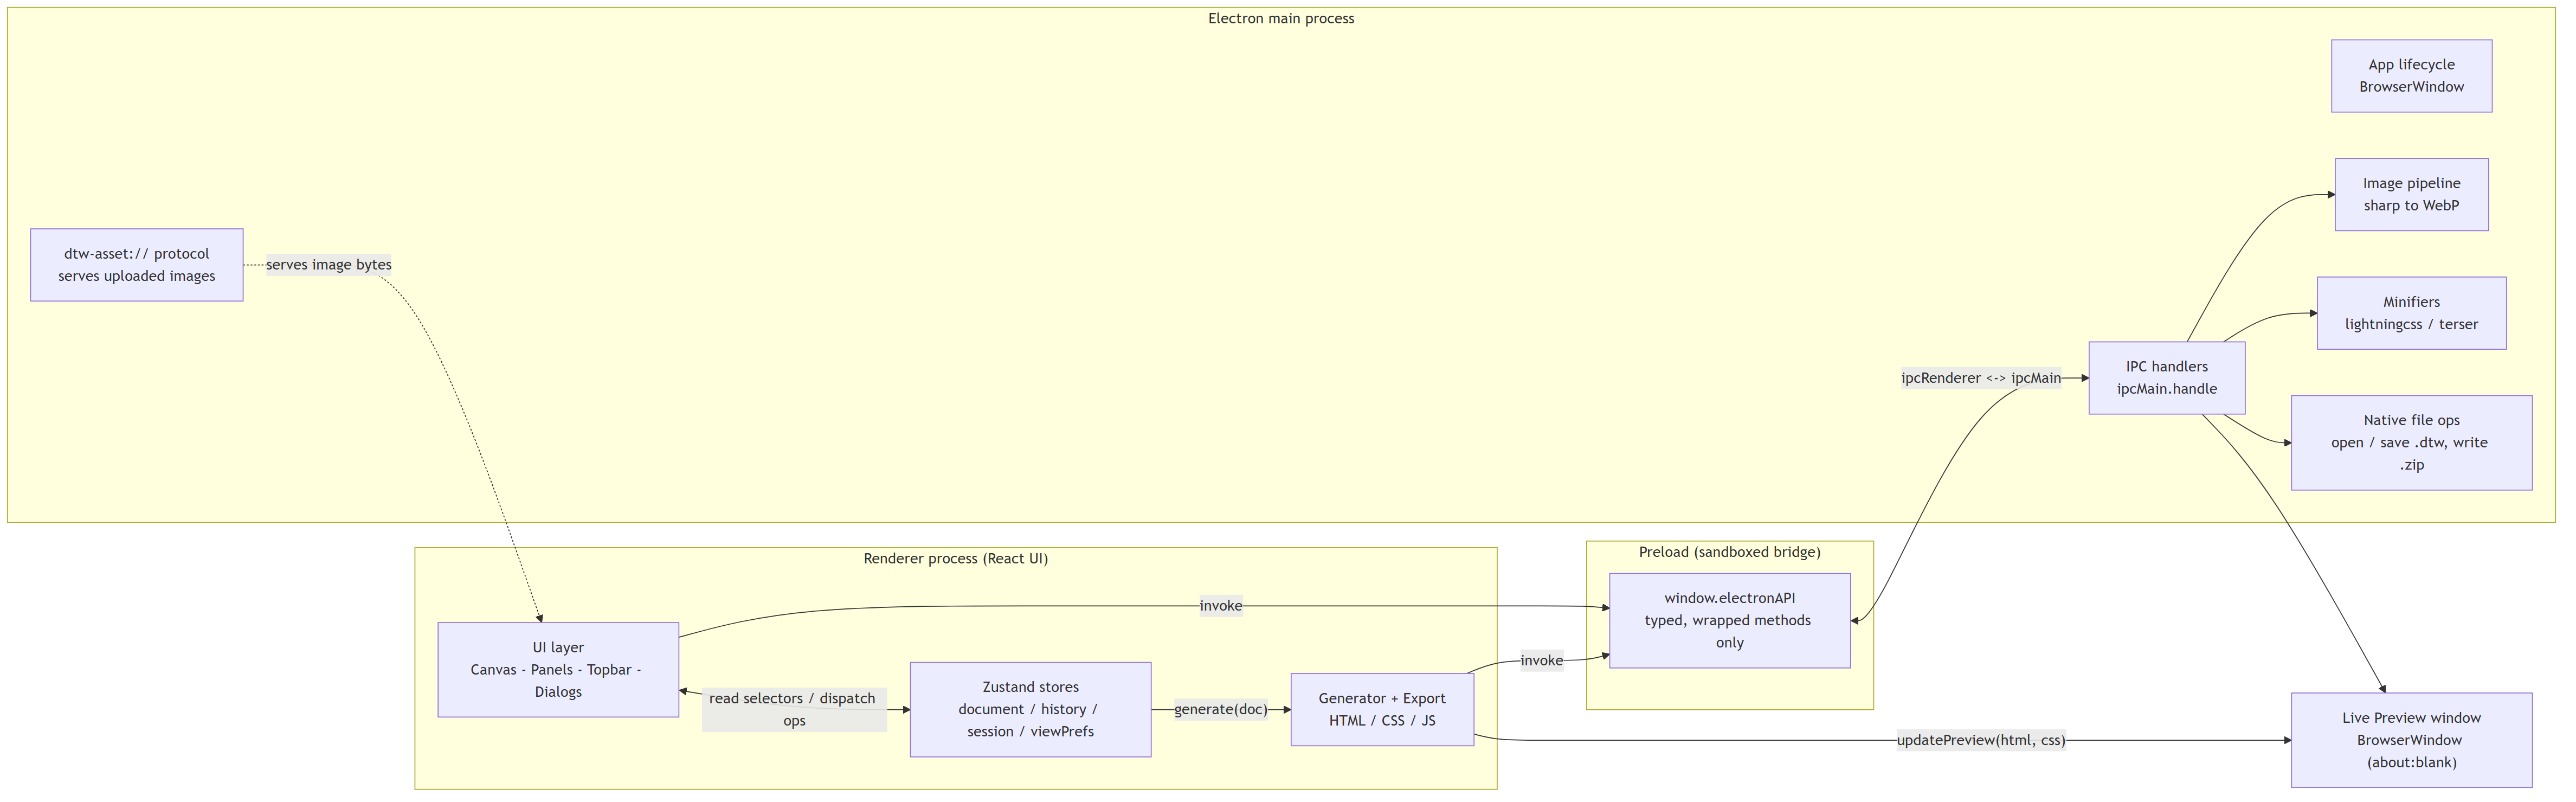
\includegraphics[width=0.92\linewidth]{01-architecture.png}
  \caption{Layered architecture: renderer (UI $\rightarrow$ store $\rightarrow$ generator) over a sandboxed preload bridge and an Electron main process.}
  \label{fig:architecture}
\end{figure}

\begin{figure}[H]
  \centering
  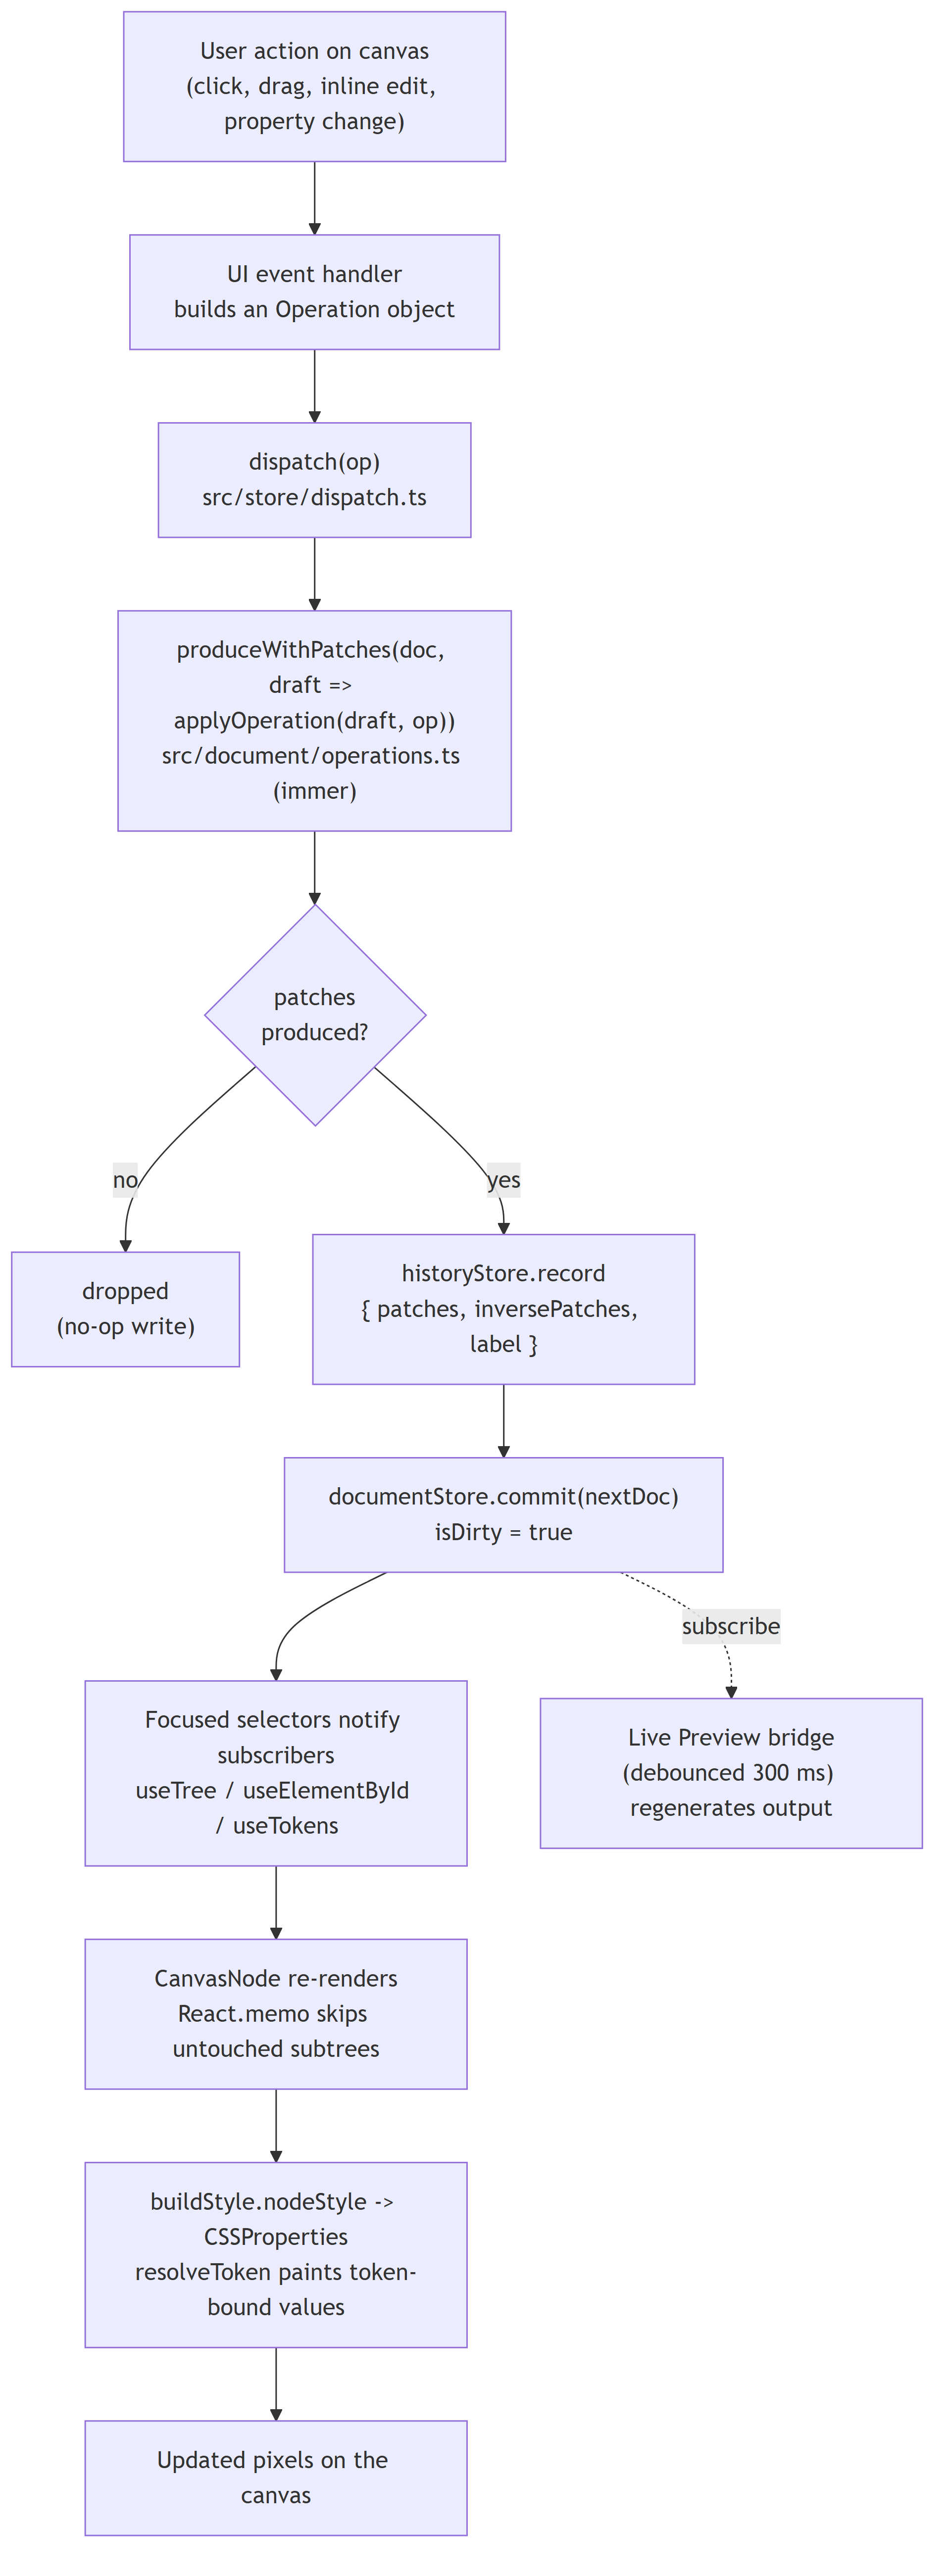
\includegraphics[width=0.92\linewidth]{02-dataflow.png}
  \caption{One-directional data flow. The UI dispatches operations to the store; the generator and export pipeline read the resulting document.}
  \label{fig:dataflow}
\end{figure}

\begin{figure}[H]
  \centering
  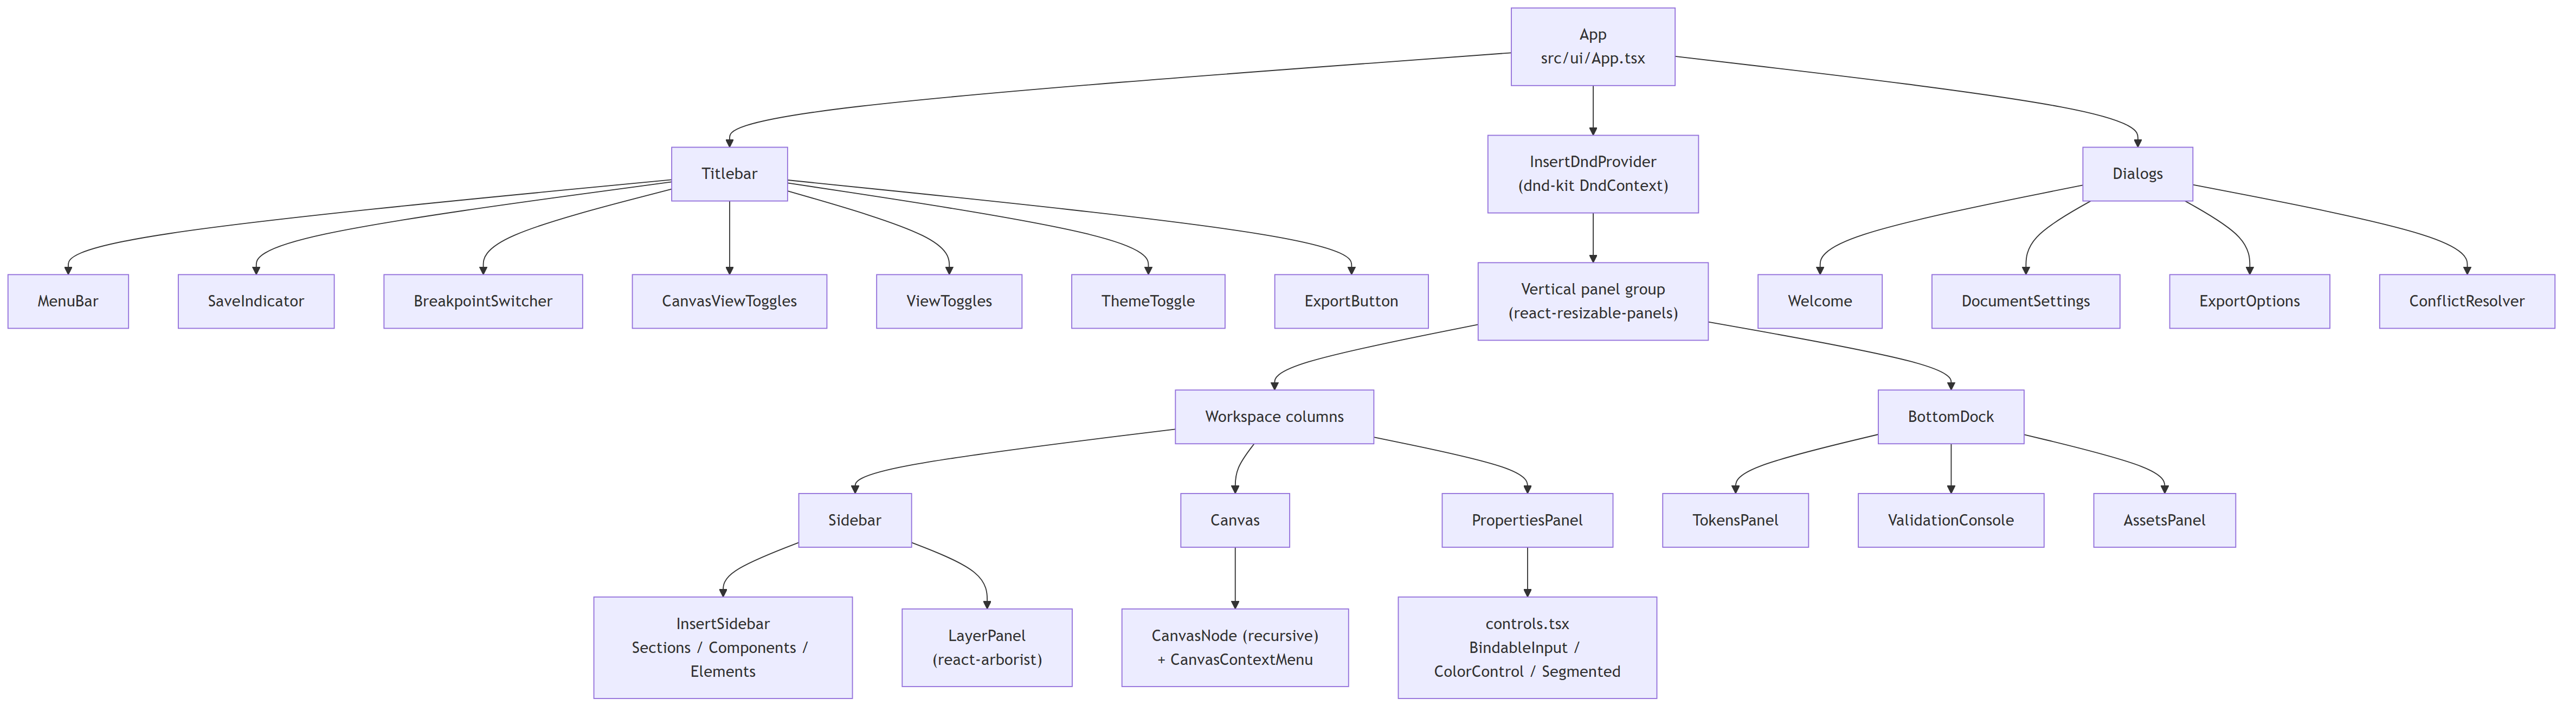
\includegraphics[width=0.86\linewidth]{04-component-hierarchy.png}
  \caption{Renderer component hierarchy.}
  \label{fig:components}
\end{figure}

\begin{figure}[H]
  \centering
  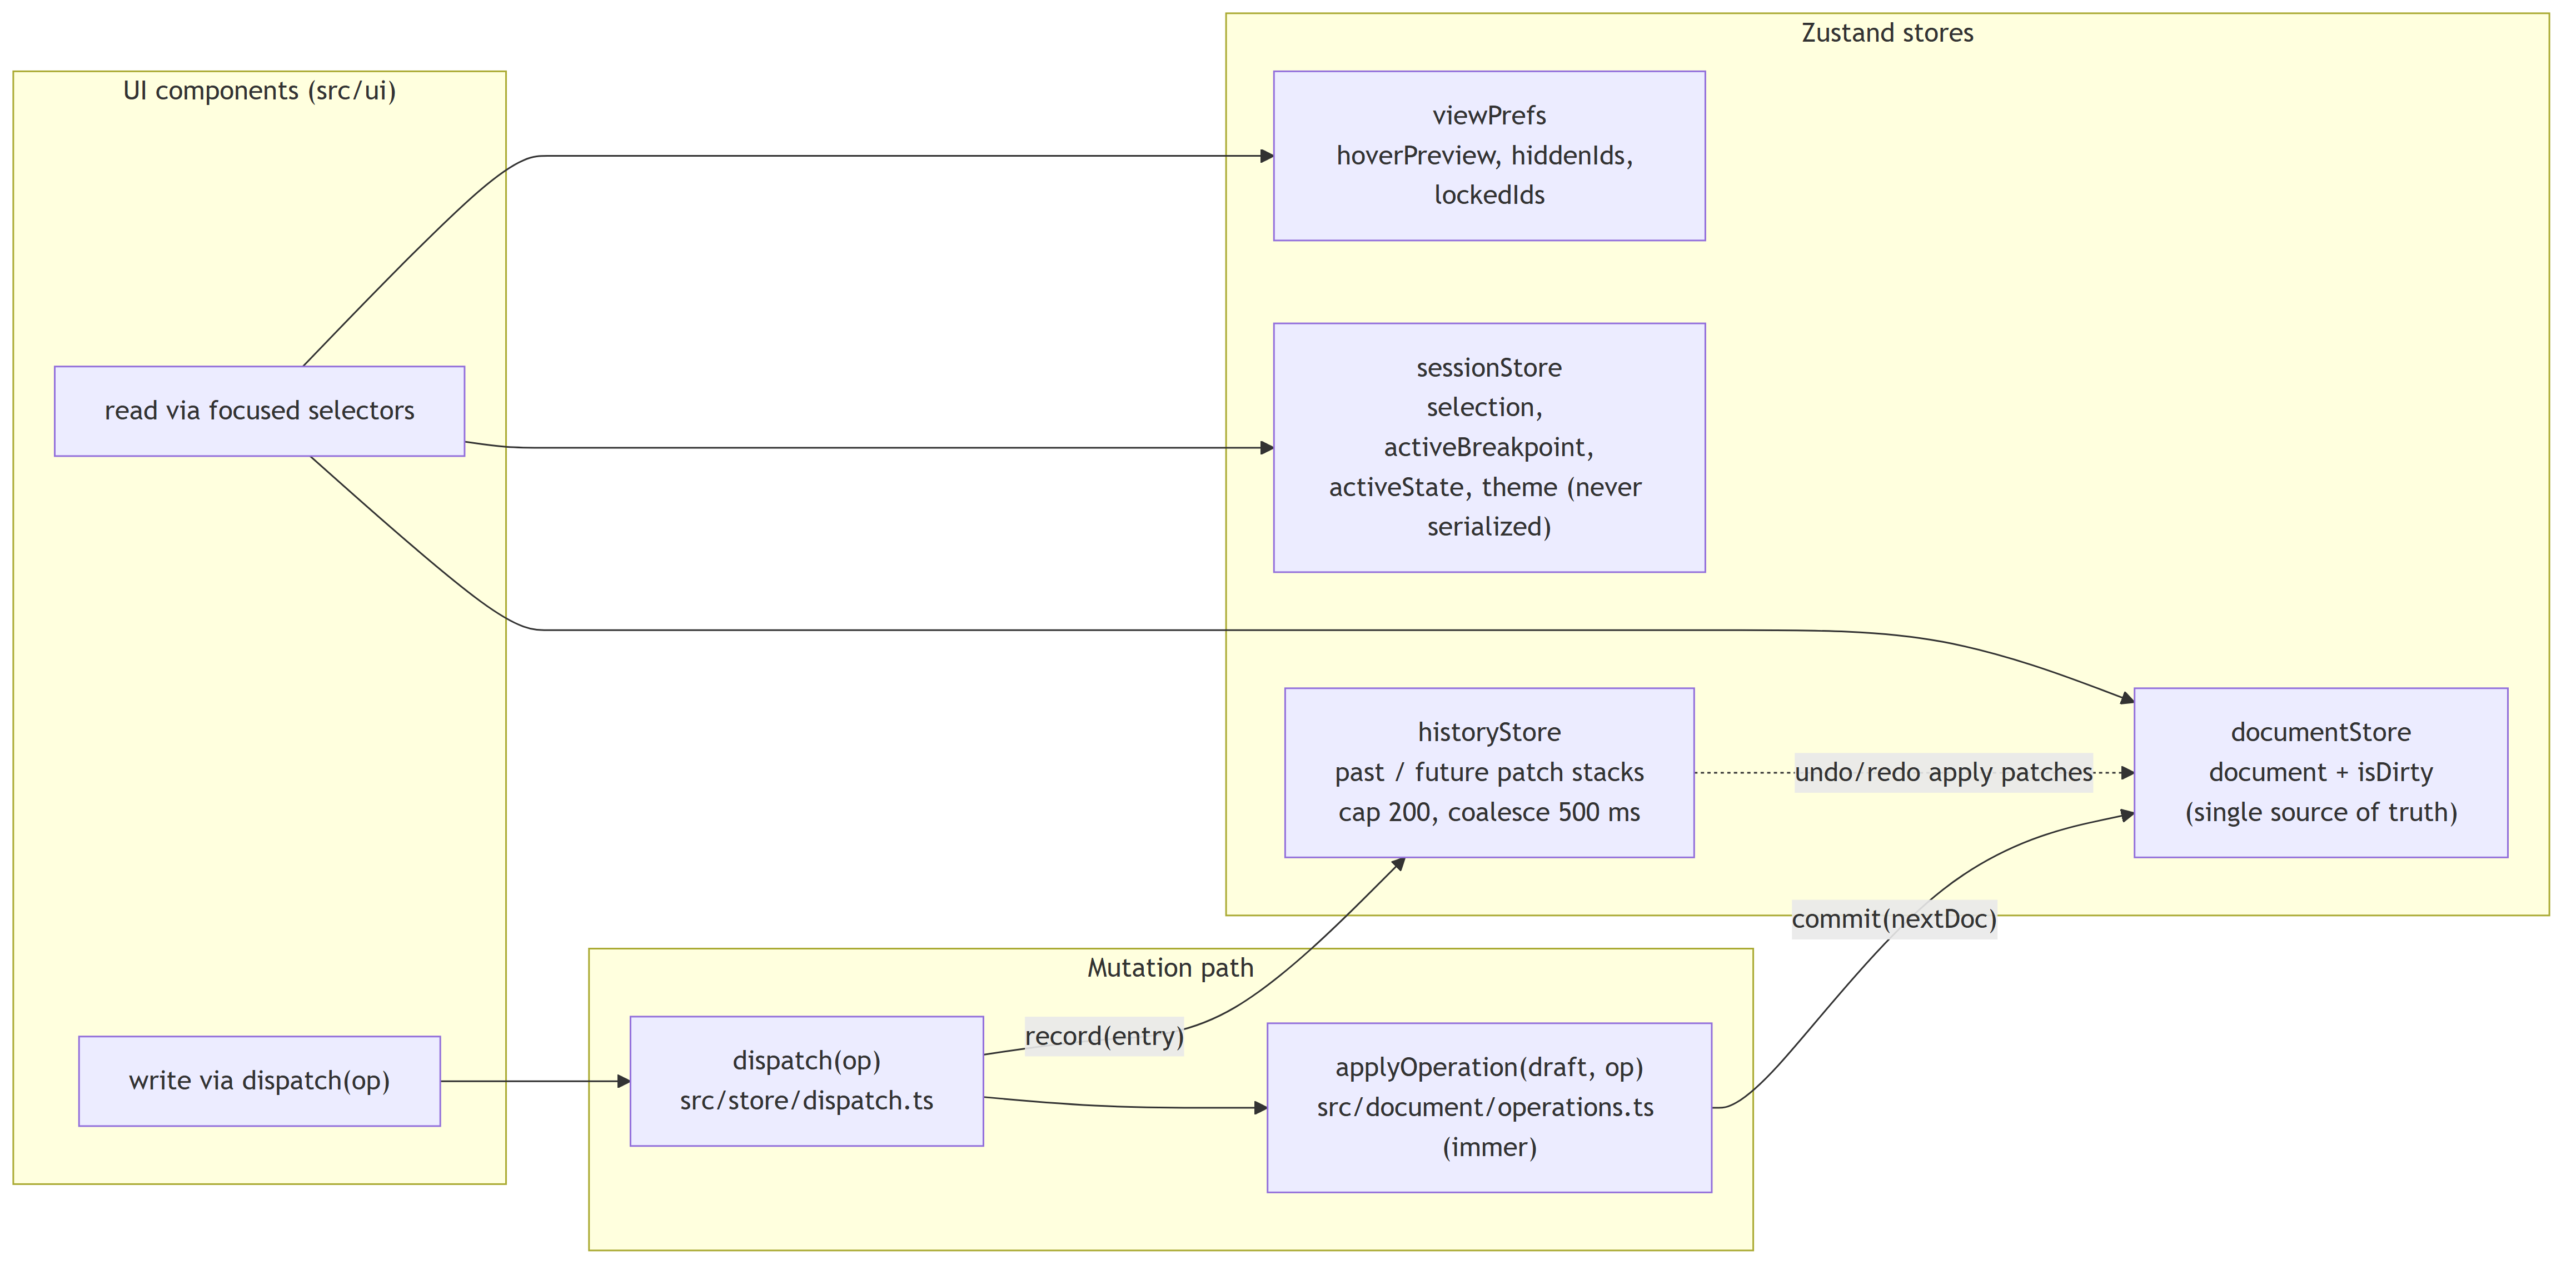
\includegraphics[width=0.78\linewidth]{05-state-stores.png}
  \caption{State stores (document, history, session) and their relationships.}
  \label{fig:stores}
\end{figure}

\section{Class Diagram (Document Model)}
The Document Model is the heart of the system and therefore its class model. A
single \texttt{Document} aggregates the design tokens, the SEO configuration, the
runtime flags, the author settings, the variables, and the asset manifest, plus one
element \texttt{tree}. Every renderable element is an \texttt{ElementNode} --- an
abstract base (all elements share an identity, a per-breakpoint \texttt{style}, a
\texttt{states} map, and an optional animation) specialised into eight concrete
primitive types. Only \texttt{ContainerNode} owns children, and its children are
themselves \texttt{ElementNode}s, which is the recursive composition that makes the
document a tree. Complex shapes (hero, cards grid, navigation) are \emph{not} new
classes: they are presets that compose these same primitives.
Figure~\ref{fig:class} shows the model, generated from
\texttt{src/document/types.ts}.

\begin{figure}[p]
  \centering
  \resizebox{\textwidth}{!}{%
  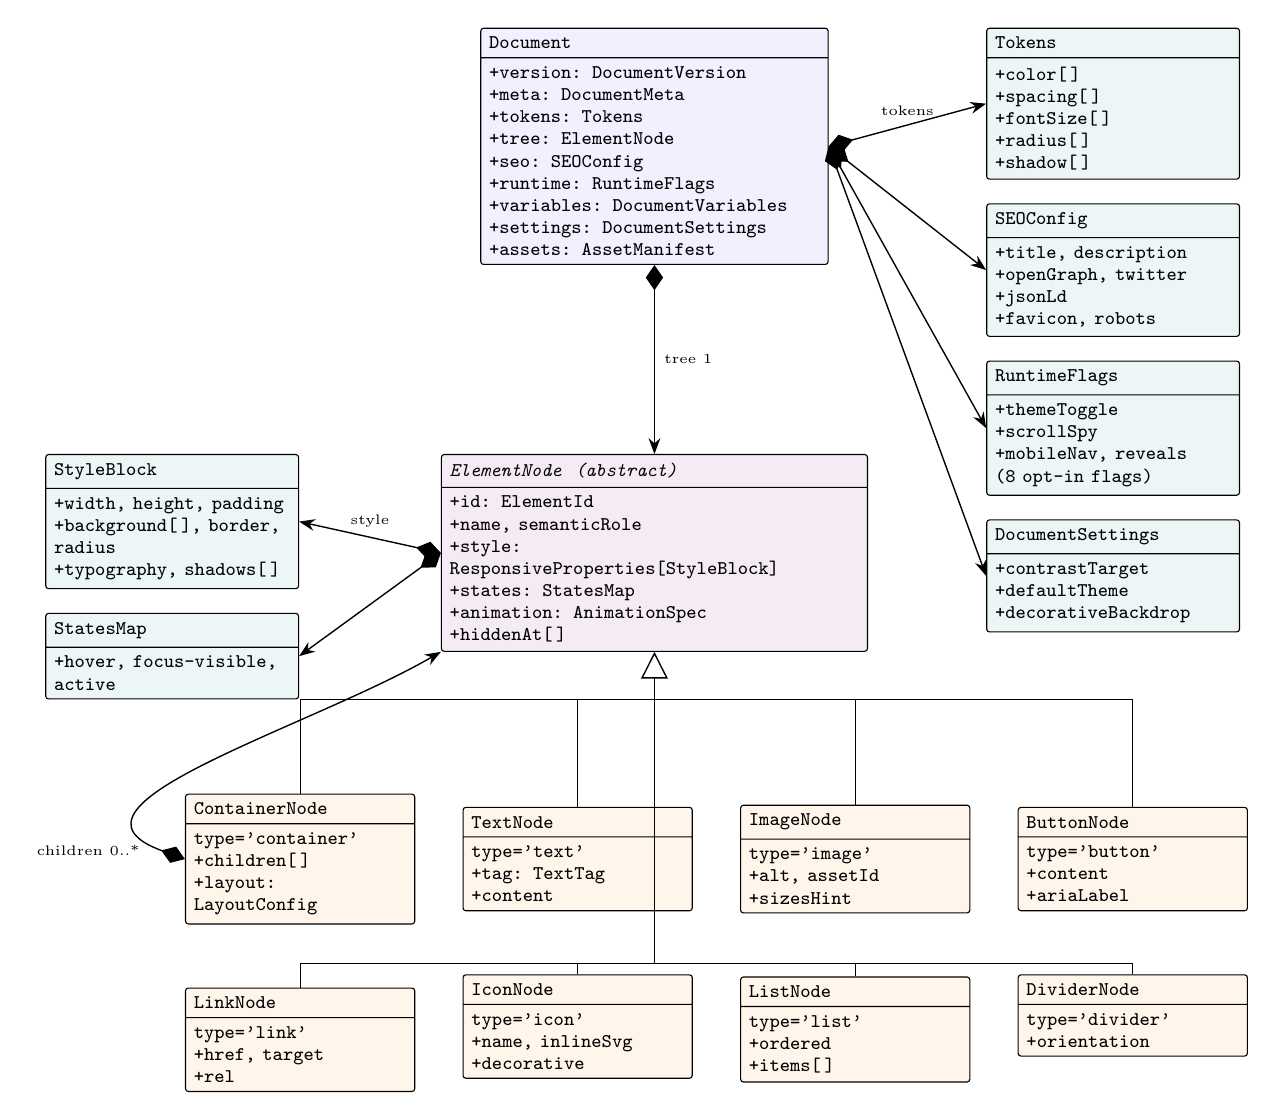
\begin{tikzpicture}[node distance=10mm and 6mm]
    % ---- Root document ----
    \node[umlclass, text width=42mm] (doc) {
      \textbf{Document}
      \nodepart{two}
      +version: DocumentVersion\\
      +meta: DocumentMeta\\
      +tokens: Tokens\\
      +tree: ElementNode\\
      +seo: SEOConfig\\
      +runtime: RuntimeFlags\\
      +variables: DocumentVariables\\
      +settings: DocumentSettings\\
      +assets: AssetManifest
    };

    % ---- Document-level value objects (right of doc) ----
    \node[umlvalue, right=20mm of doc.north east, anchor=north west] (tokens) {
      \textbf{Tokens}\nodepart{two}+color[\,]\\+spacing[\,]\\+fontSize[\,]\\+radius[\,]\\+shadow[\,]
    };
    \node[umlvalue, below=3mm of tokens] (seo) {
      \textbf{SEOConfig}\nodepart{two}+title, description\\+openGraph, twitter\\+jsonLd\\+favicon, robots
    };
    \node[umlvalue, below=3mm of seo] (runtime) {
      \textbf{RuntimeFlags}\nodepart{two}+themeToggle\\+scrollSpy\\+mobileNav, reveals\\(8 opt-in flags)
    };
    \node[umlvalue, below=3mm of runtime] (settings) {
      \textbf{DocumentSettings}\nodepart{two}+contrastTarget\\+defaultTheme\\+decorativeBackdrop
    };

    % ---- Abstract element ----
    \node[umlabstract, below=24mm of doc, text width=52mm] (en) {
      \textit{\textbf{ElementNode}}\, \textit{(abstract)}
      \nodepart{two}
      +id: ElementId\\
      +name, semanticRole\\
      +style: ResponsiveProperties[StyleBlock]\\
      +states: StatesMap\\
      +animation: AnimationSpec\\
      +hiddenAt[\,]
    };

    % ---- Element-level value objects (LEFT of en; kept compact so the recursive
    %      "children" edge has a clear corridor below them) ----
    \node[umlvalue, left=18mm of en.north west, anchor=north east] (style) {
      \textbf{StyleBlock}\nodepart{two}+width, height, padding\\+background[\,], border, radius\\+typography, shadows[\,]
    };
    \node[umlvalue, below=3mm of style] (states) {
      \textbf{StatesMap}\nodepart{two}+hover, focus-visible, active
    };

    % ---- Concrete subclasses: two rows of four ----
    \node[umlnode, below=18mm of en, xshift=-45mm] (c1) {\textbf{ContainerNode}\nodepart{two}type='container'\\+children[\,]\\+layout: LayoutConfig};
    \node[umlnode, right=6mm of c1] (c2) {\textbf{TextNode}\nodepart{two}type='text'\\+tag: TextTag\\+content};
    \node[umlnode, right=6mm of c2] (c3) {\textbf{ImageNode}\nodepart{two}type='image'\\+alt, assetId\\+sizesHint};
    \node[umlnode, right=6mm of c3] (c4) {\textbf{ButtonNode}\nodepart{two}type='button'\\+content\\+ariaLabel};
    \node[umlnode, below=8mm of c1] (c5) {\textbf{LinkNode}\nodepart{two}type='link'\\+href, target\\+rel};
    \node[umlnode, below=8mm of c2] (c6) {\textbf{IconNode}\nodepart{two}type='icon'\\+name, inlineSvg\\+decorative};
    \node[umlnode, below=8mm of c3] (c7) {\textbf{ListNode}\nodepart{two}type='list'\\+ordered\\+items[\,]};
    \node[umlnode, below=8mm of c4] (c8) {\textbf{DividerNode}\nodepart{two}type='divider'\\+orientation};

    % ---- Compositions from Document ----
    \draw[compose] (doc.east) -- (tokens.west) node[midway, above, font=\tiny]{tokens};
    \draw[compose] (doc.east) -- (seo.west);
    \draw[compose] (doc.east) -- (runtime.west);
    \draw[compose] (doc.east) -- (settings.west);
    \draw[compose] (doc.south) -- (en.north) node[midway, right, font=\tiny]{tree 1};

    % ---- Compositions on the element (to the left) ----
    \draw[compose] (en.west) -- (style.east) node[midway, above, font=\tiny]{style};
    \draw[compose] (en.west) -- (states.east);

    % ---- Generalisation (nested shared bus) ----
    \coordinate (pbus) at ($(en.south)+(0,-6mm)$);
    \draw[inherit] (pbus) -- (en.south);
    \draw (c1.north |- pbus) -- (c4.north |- pbus);
    \foreach \c in {c1,c2,c3,c4}{ \draw (\c.north) -- (\c.north |- pbus); }
    \coordinate (r2y) at ($(c5.north)+(0,3mm)$);
    \draw (en.south |- pbus) -- (en.south |- r2y);
    \draw (c5.north |- r2y) -- (c8.north |- r2y);
    \foreach \c in {c5,c6,c7,c8}{ \draw (\c.north) -- (\c.north |- r2y); }

    % ---- Recursive composition: Container owns ElementNode children ----
    \draw[compose] (c1.west) to[out=160, in=210, looseness=1.2]
      node[pos=0.12, below left=-0.5mm and 0mm, font=\tiny, align=right]{children 0..*} (en.south west);
  \end{tikzpicture}%
  }
  \caption{Class diagram of the Document Model. Filled diamonds denote composition; the hollow triangle denotes generalisation. \texttt{ContainerNode} composes further \texttt{ElementNode}s, making the document a recursive tree.}
  \label{fig:class}
\end{figure}

\section{Use-Case Diagram}
The system has two actors: the \emph{Author}, a human working in the graphical
editor, and the \emph{MCP Client}, a program or agent driving the same pipeline
headlessly. Figure~\ref{fig:usecase} shows their goals. Note that both
\emph{Author \& export a page} and \emph{Drive builder headlessly} \emph{include}
the shared \emph{Validate document} and \emph{Export ZIP bundle} use cases --- the
same generation, accessibility gate, and packaging serve both the interactive and
the headless path.

\begin{figure}[H]
  \centering
  \resizebox{0.98\textwidth}{!}{%
  \begin{tikzpicture}
    % ---- Use cases: left column ----
    \node[usecase] (uc1) {Author \& export\\a page};
    \node[usecase, below=6mm of uc1] (uc2) {Draw to create\\an element};
    \node[usecase, below=6mm of uc2] (uc3) {Match my\\layout};
    \node[usecase, below=6mm of uc3] (uc5) {Save / open \&\\recover project};
    % ---- Use cases: right column ----
    \node[usecase, right=26mm of uc1] (ucA) {Insert / edit\\elements};
    \node[usecase, below=6mm of ucA] (ucB) {Manage tokens\\\& theme};
    \node[usecase, below=6mm of ucB] (ucV) {Validate\\document};
    \node[usecase, below=6mm of ucV] (ucE) {Export ZIP\\bundle};
    \node[usecase, below=6mm of ucE] (ucH) {Drive builder\\headlessly};
    % ---- System boundary ----
    \node[draw, thick, rounded corners, fit=(uc1)(uc5)(ucA)(ucH),
      inner sep=7mm, label={[font=\bfseries]above:Draw-to-Web}] (sys) {};
    % ---- Actors ----
    \coordinate (author) at ($(uc3.west)+(-40mm,10mm)$);
    \pic at (author) {ucactor};
    \node[font=\footnotesize, below=15mm of author] {Author};
    \coordinate (mcp) at ($(ucH.east)+(40mm,0mm)$);
    \pic at (mcp) {ucactor};
    \node[font=\footnotesize, below=15mm of mcp, align=center] {MCP\\Client};
    % ---- Associations (Author) ----
    \foreach \u in {uc1,uc2,uc3,uc5,ucA,ucB}{ \draw[ucedge] (author) -- (\u.west); }
    % ---- Associations (MCP client) ----
    \draw[ucedge] (mcp) -- (ucH.east);
    % ---- Includes ----
    \draw[ucinclude] (uc1) -- (ucV) node[midway, above, font=\tiny, sloped]{\guillemotleft include\guillemotright};
    \draw[ucinclude] (ucH) to[out=150,in=270] node[pos=0.5, right, font=\tiny]{\guillemotleft include\guillemotright} (ucE.south);
    \draw[ucinclude] (ucH) to[out=120,in=250] (ucV.south);
    \draw[ucinclude] (uc1) to[out=-20,in=160] node[pos=0.5, below, font=\tiny]{\guillemotleft include\guillemotright} (ucE.west);
  \end{tikzpicture}%
  }
  \caption{Use-case diagram. The Author drives the graphical goals; the MCP Client drives the headless goal. Both the interactive and headless export paths \guillemotleft include\guillemotright{} the same validation and packaging.}
  \label{fig:usecase}
\end{figure}

\section{Sequence Diagrams}
Two interactions best characterise the system. The first,
Figure~\ref{fig:seqdraw}, is \emph{draw-to-create}: how a rectangle drawn on the
canvas becomes a real element through an ordinary operation, so that the drawn
pixels themselves never enter the store. The second, Figure~\ref{fig:seqexport}, is
the \emph{export pipeline}: how a document is validated, generated, gated for
accessibility, optimised across the IPC boundary, and packaged. The nine-stage
pipeline is also shown as a flow in Figure~\ref{fig:exportflow}.

\begin{figure}[H]
  \centering
  \resizebox{\textwidth}{!}{%
  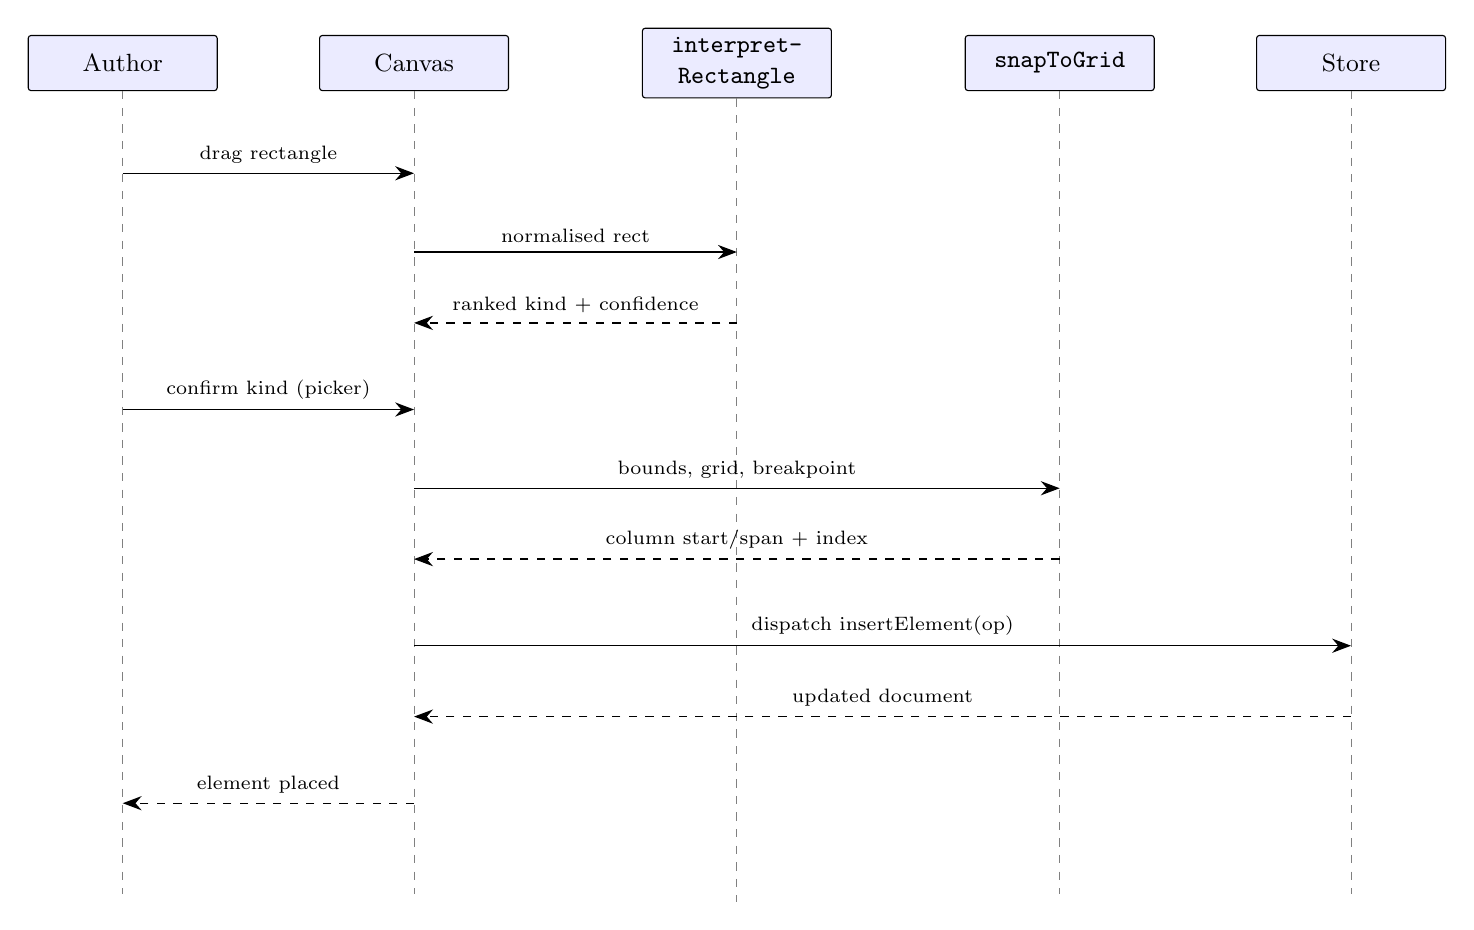
\begin{tikzpicture}
    % participants
    \node[seqbox] (p1) at (0,0)    {Author};
    \node[seqbox] (p2) at (37mm,0) {Canvas};
    \node[seqbox] (p3) at (78mm,0) {\texttt{interpret-}\\\texttt{Rectangle}};
    \node[seqbox] (p4) at (119mm,0){\texttt{snapToGrid}};
    \node[seqbox] (p5) at (156mm,0){Store};
    % lifelines
    \foreach \p in {p1,p2,p3,p4,p5}{ \draw[lifeline] (\p.south) -- ($(\p.south)+(0,-102mm)$); }
    % message y-levels
    \foreach \i/\y in {1/-14,2/-24,3/-33,4/-44,5/-54,6/-63,7/-74,8/-83,9/-94}{
      \coordinate (m\i) at (0,\y mm); }
    % messages
    \draw[seqmsg] (p1 |- m1) -- (p2 |- m1) node[midway, above, font=\scriptsize]{drag rectangle};
    \draw[seqmsg] (p2 |- m2) -- (p3 |- m2) node[midway, above, font=\scriptsize]{normalised rect};
    \draw[seqret] (p3 |- m3) -- (p2 |- m3) node[midway, above, font=\scriptsize]{ranked kind + confidence};
    \draw[seqmsg] (p1 |- m4) -- (p2 |- m4) node[midway, above, font=\scriptsize]{confirm kind (picker)};
    \draw[seqmsg] (p2 |- m5) -- (p4 |- m5) node[midway, above, font=\scriptsize]{bounds, grid, breakpoint};
    \draw[seqret] (p4 |- m6) -- (p2 |- m6) node[midway, above, font=\scriptsize]{column start/span + index};
    \draw[seqmsg] (p2 |- m7) -- (p5 |- m7) node[midway, above, font=\scriptsize]{dispatch insertElement(op)};
    \draw[seqret] (p5 |- m8) -- (p2 |- m8) node[midway, above, font=\scriptsize]{updated document};
    \draw[seqret] (p2 |- m9) -- (p1 |- m9) node[midway, above, font=\scriptsize]{element placed};
  \end{tikzpicture}%
  }
  \caption{Sequence diagram: draw-to-create. The canvas interprets the rectangle and snaps it to a grid placement (pure functions), then dispatches a normal \texttt{insertElement} operation; the drawn pixels never enter the store.}
  \label{fig:seqdraw}
\end{figure}

\begin{figure}[H]
  \centering
  \resizebox{\textwidth}{!}{%
  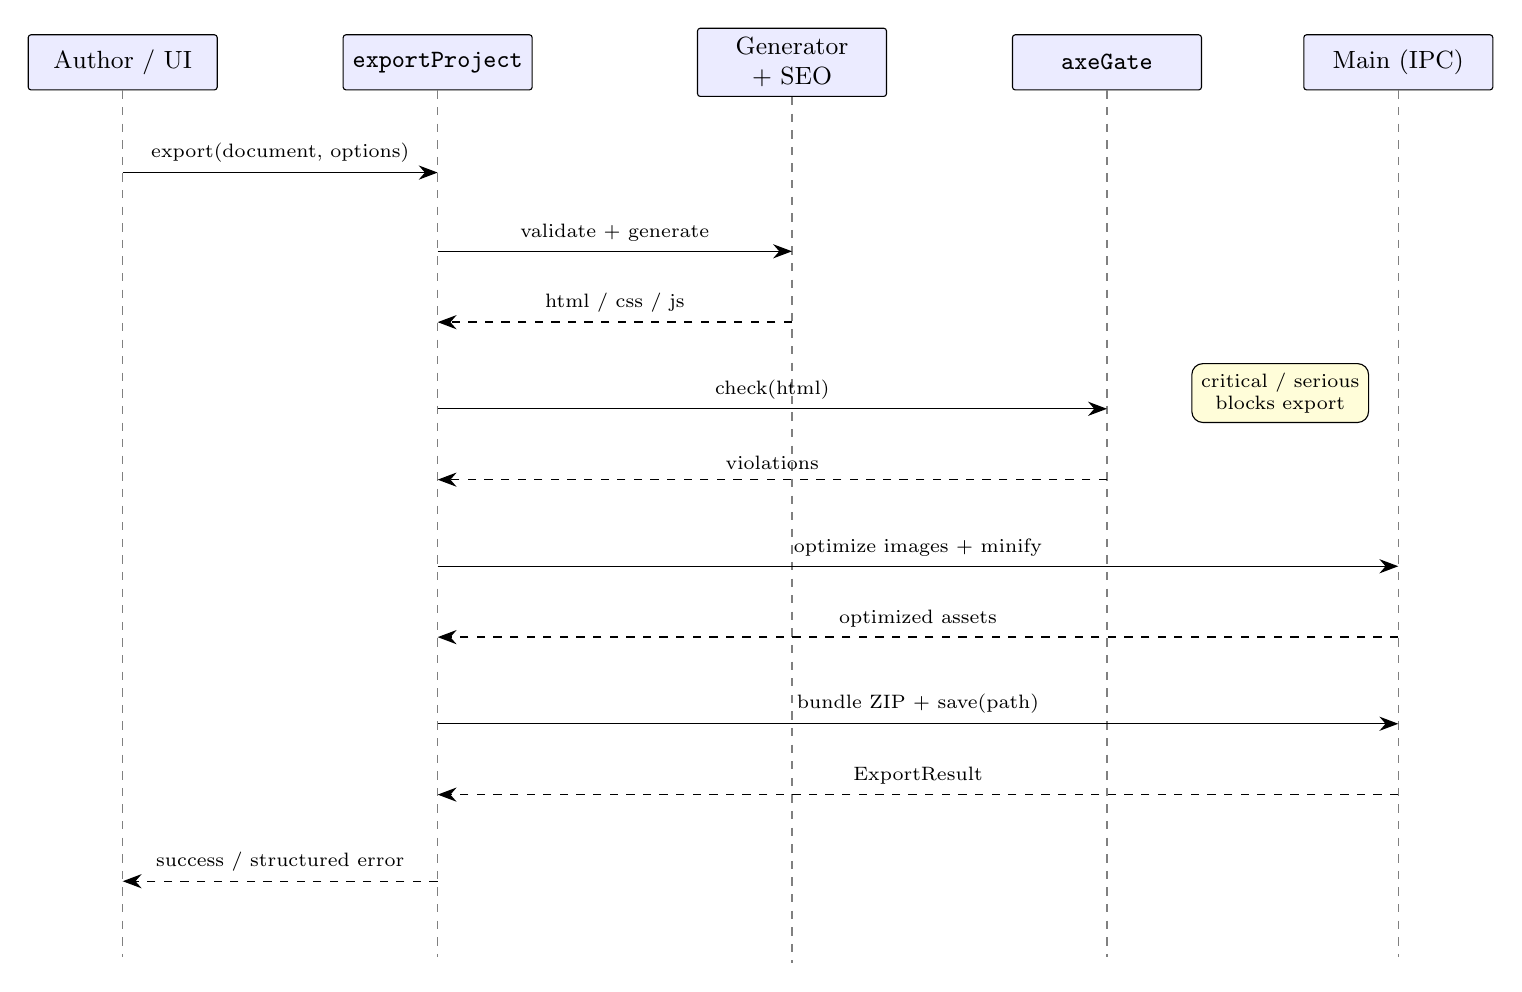
\begin{tikzpicture}
    % participants
    \node[seqbox] (p1) at (0,0)    {Author / UI};
    \node[seqbox] (p2) at (40mm,0) {\texttt{exportProject}};
    \node[seqbox] (p3) at (85mm,0) {Generator\\+ SEO};
    \node[seqbox] (p4) at (125mm,0){\texttt{axeGate}};
    \node[seqbox] (p5) at (162mm,0){Main (IPC)};
    % lifelines
    \foreach \p in {p1,p2,p3,p4,p5}{ \draw[lifeline] (\p.south) -- ($(\p.south)+(0,-110mm)$); }
    % message y-levels
    \foreach \i/\y in {1/-14,2/-24,3/-33,4/-44,5/-53,6/-64,7/-73,8/-84,9/-93,10/-104}{
      \coordinate (m\i) at (0,\y mm); }
    \draw[seqmsg] (p1 |- m1) -- (p2 |- m1) node[midway, above, font=\scriptsize]{export(document, options)};
    \draw[seqmsg] (p2 |- m2) -- (p3 |- m2) node[midway, above, font=\scriptsize]{validate + generate};
    \draw[seqret] (p3 |- m3) -- (p2 |- m3) node[midway, above, font=\scriptsize]{html / css / js};
    \draw[seqmsg] (p2 |- m4) -- (p4 |- m4) node[midway, above, font=\scriptsize]{check(html)};
    \draw[seqret] (p4 |- m5) -- (p2 |- m5) node[midway, above, font=\scriptsize]{violations};
    \draw[seqmsg] (p2 |- m6) -- (p5 |- m6) node[midway, above, font=\scriptsize]{optimize images + minify};
    \draw[seqret] (p5 |- m7) -- (p2 |- m7) node[midway, above, font=\scriptsize]{optimized assets};
    \draw[seqmsg] (p2 |- m8) -- (p5 |- m8) node[midway, above, font=\scriptsize]{bundle ZIP + save(path)};
    \draw[seqret] (p5 |- m9) -- (p2 |- m9) node[midway, above, font=\scriptsize]{ExportResult};
    \draw[seqret] (p2 |- m10) -- (p1 |- m10) node[midway, above, font=\scriptsize]{success / structured error};
    % a11y note (placed in whitespace right of the gate, above the minify message)
    \node[draw, fill=yellow!15, font=\scriptsize, align=center, rounded corners]
      at (147mm,-42mm) {critical / serious\\blocks export};
  \end{tikzpicture}%
  }
  \caption{Sequence diagram: the export pipeline. The accessibility gate runs before any asset crosses the IPC boundary; a critical or serious violation aborts the export with a structured error.}
  \label{fig:seqexport}
\end{figure}

\begin{figure}[H]
  \centering
  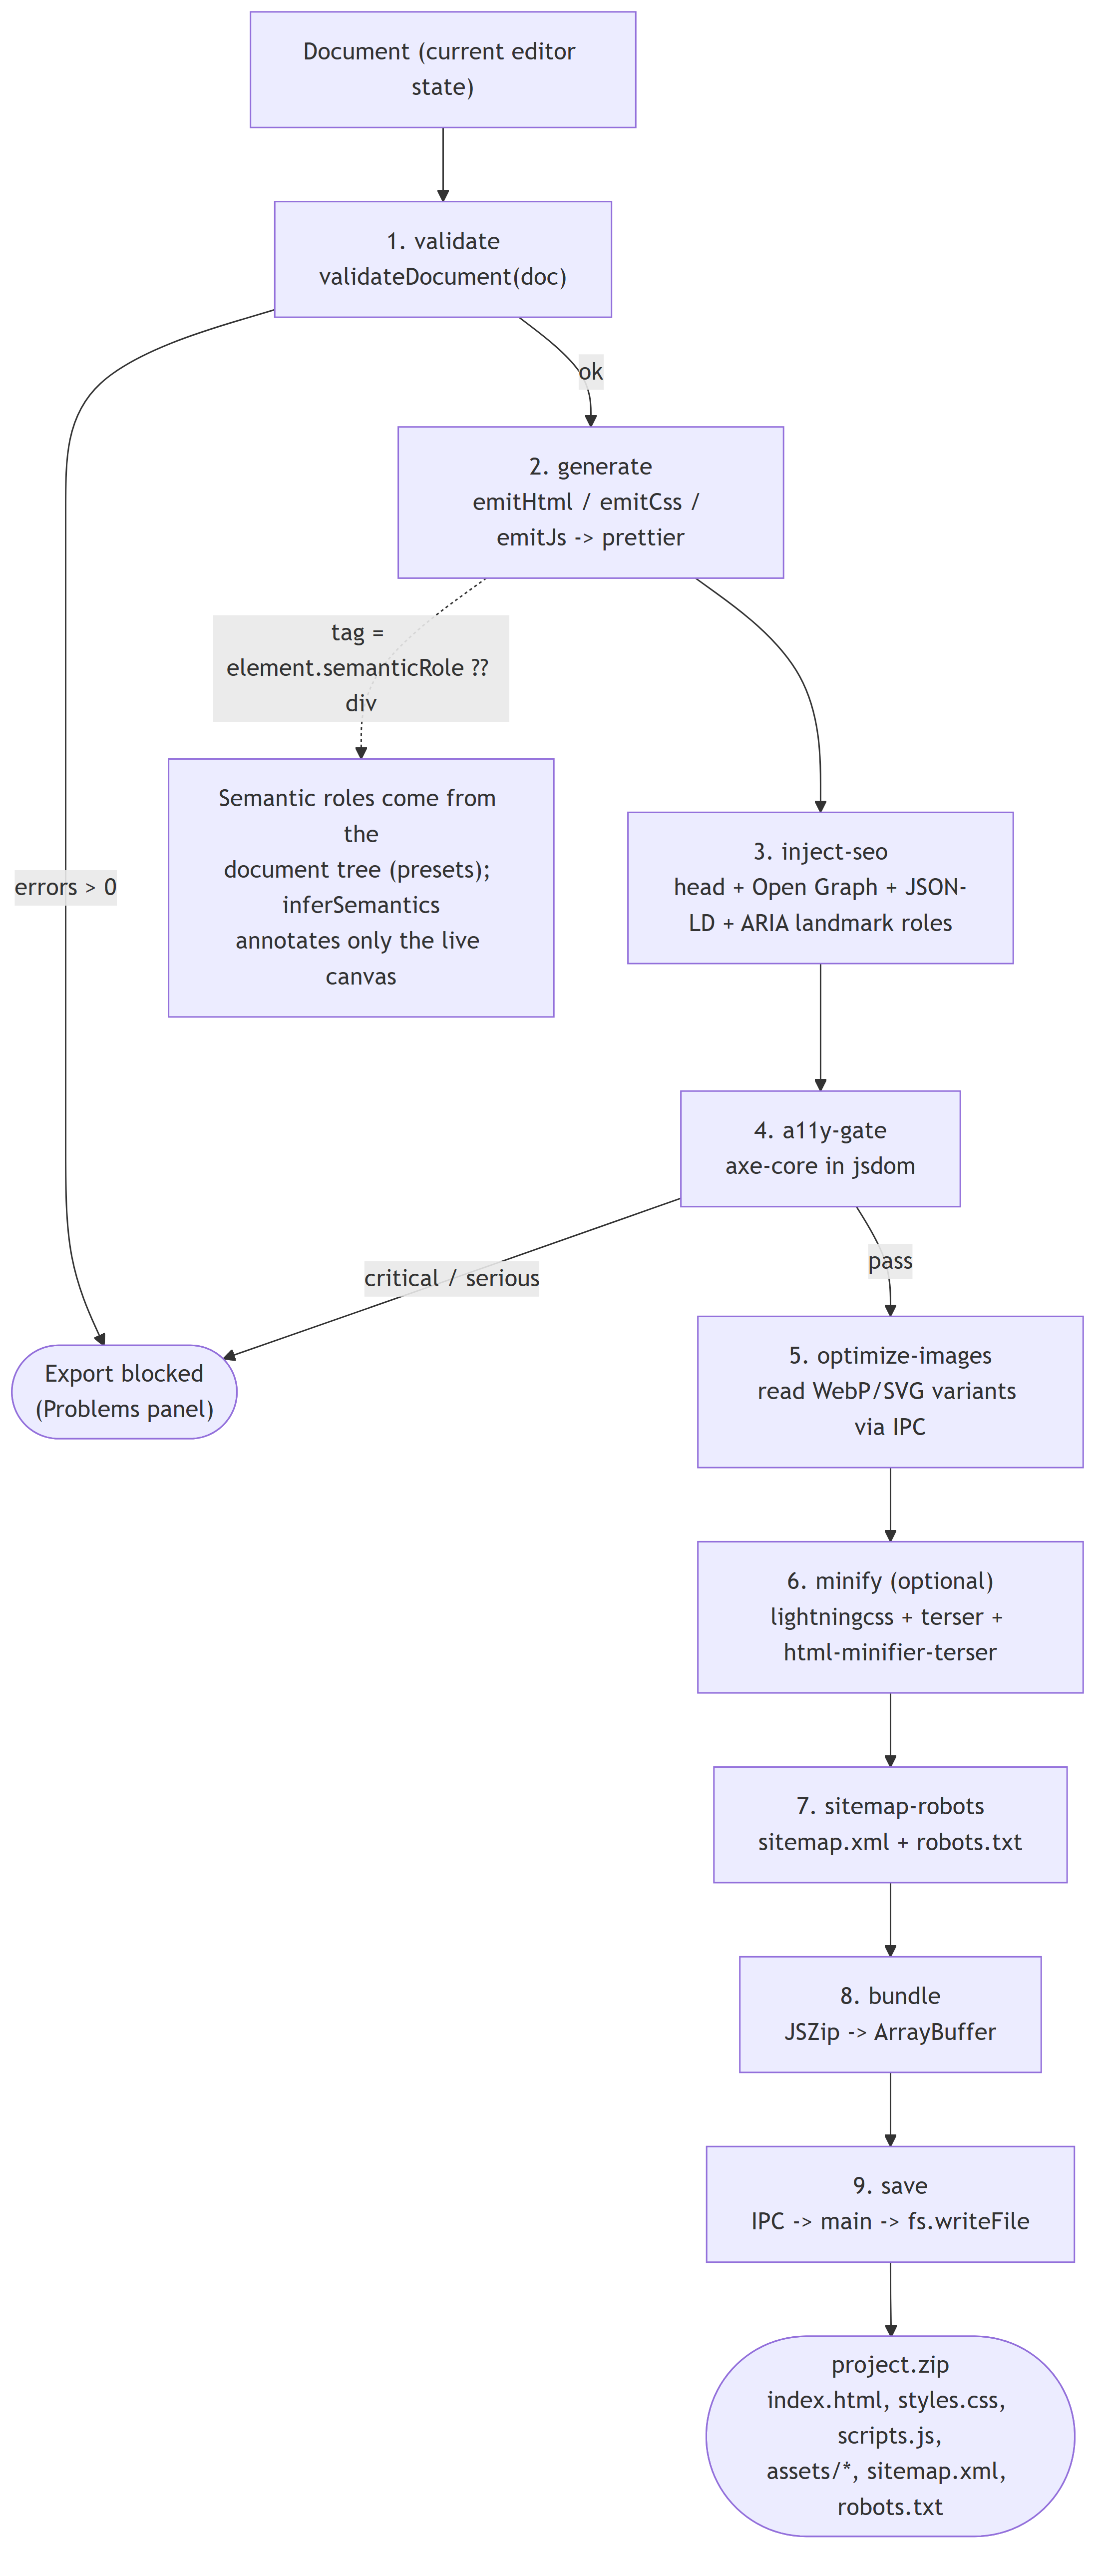
\includegraphics[width=0.92\linewidth]{03-export-pipeline.png}
  \caption{The nine-stage export pipeline as a flow: validate $\rightarrow$ generate $\rightarrow$ inject-SEO $\rightarrow$ a11y-gate $\rightarrow$ optimize-images $\rightarrow$ minify $\rightarrow$ sitemap/robots $\rightarrow$ bundle $\rightarrow$ save.}
  \label{fig:exportflow}
\end{figure}

% SOURCES: README.md (Stack); CLAUDE.md (Tech Stack); docs/0.2.0v/plan.md
%          (§9 Library-to-Feature Map — the JUSTIFICATION source);
%          docs/1.0.0v/supervisor-report.md

\chapter{Technologies Used}
\label{ch:tech}

\section{Overview}
The application is a single TypeScript codebase spanning three runtime contexts:
an Electron \emph{main} process (privileged, native OS access), a \emph{preload}
security bridge, and a React \emph{renderer} (the editor UI). It is built and
packaged with Vite and electron-builder. Every technology was chosen against a
specific requirement rather than by default; Table~\ref{tab:tech} lists the
principal choices and the reason for each, and the sections that follow expand on
the choices that best show the engineering rationale.

\begin{table}[H]
  \centering
  \caption{Principal technologies and justification.}
  \label{tab:tech}
  \small
  \begin{tabularx}{\linewidth}{@{}l l X@{}}
    \toprule
    \textbf{Technology} & \textbf{Role} & \textbf{Justification} \\
    \midrule
    Electron \cite{electron} & Desktop shell & Cross-platform desktop with native file access; local-first, no server required. \\
    React 18 \cite{react} & UI & Declarative rendering of the document tree; mature ecosystem and tooling. \\
    TypeScript 5 \cite{typescript} & Language & Strict typing across three processes; the cross-owner contracts are enforced at compile time. \\
    Zustand + immer \cite{zustand,immer} & State + history & Minimal store with no boilerplate; \texttt{immer} patches yield undo/redo almost for free. \\
    Zod \cite{zod} & Validation & Schema validation at the IPC and file-load boundaries; types are derived via \texttt{z.infer} to keep schema and type in lockstep. \\
    axe-core \cite{axecore} & A11y gate & Industry-standard accessibility engine; blocks export on any critical or serious issue. \\
    prettier \cite{prettier} & Output format & Formats generated HTML/CSS so it reads as hand-written before minification. \\
    Lightning CSS \cite{lightningcss} & CSS minify & Fast, correct CSS transform and minification in the export pipeline. \\
    sharp \cite{sharp} & Images & Generates WebP and \texttt{srcset} variants in the main process. \\
    Vite \cite{vite} & Build / dev & Fast hot-module-reload dev server and production bundling. \\
    MCP SDK \cite{mcp-spec} & Headless API & Exposes the pipeline as tools to agents and clients over \texttt{stdio}. \\
    \bottomrule
  \end{tabularx}
\end{table}

Beyond the principals, the editor uses \texttt{@dnd-kit} for canvas drag-and-drop
and \texttt{react-arborist} for the layers tree; Radix UI primitives for accessible
tabs, dialogs, and popovers; \texttt{react-colorful} and \texttt{chroma-js} for the
colour picker and contrast checks; and \texttt{jszip} plus
\texttt{html-minifier-terser} in the export pipeline. Each of these maps to a
specific Tier-1 feature in the execution plan's library-to-feature justification.

\section{Selected Justifications in Depth}

\subsection*{Why a single Document Model backed by immer}
Making one immutable \texttt{Document} the source of truth means that undo/redo,
persistence, and generation all reduce to functions of one value. \texttt{immer}
is what makes this ergonomic: each operation is written as if it were mutating a
draft, while \texttt{produceWithPatches} captures the forward and inverse patches
that the history store replays for undo and redo. The operations therefore never
need to know anything about history --- reversibility is a property of the patch
round-trip, not of the operation code.

\subsection*{Why an accessibility hard gate rather than a linter}
Accessibility is treated as a build \emph{error}, not a warning. The
\texttt{axe-core} engine runs on the generated HTML inside a \texttt{jsdom}
document, and any critical or serious violation aborts the export. This guarantees
a compliance floor that no manual review process could match consistently, and ---
crucially --- it applies to \emph{every} export path, including the headless MCP
server, so the guarantee cannot be bypassed by scripting the tool.

\subsection*{Why prettier plus stable identifiers gives deterministic output}
A recurring requirement is that identical input must yield byte-identical output.
Two decisions make this hold: element identifiers are generated once and are stable
across save/load (they are never regenerated), and the generator emits no
timestamps or random values. Running the emitted HTML and CSS through
\texttt{prettier} then produces a canonical, human-readable form, so two exports of
the same document are not merely equivalent but textually identical --- which makes
the output diff-able and the pipeline testable by exact comparison.

% SOURCES: docs/0.2.0v/architecture.md; docs/0.2.0v/element-model.md;
%          docs/1.0.0v/supervisor-report.md (§4–§6, §5a); README.md;
%          src/document/*, src/generator/*, src/export/*, src/draw/*, src/match/*, mcp/*

\chapter{Implementation}
\label{ch:impl}

This chapter describes how the system was built, following the data as it flows
from the Document Model through the generator to the export pipeline, and then the
three v1.0.0 authoring surfaces and the security boundary.

\section{The Document Model}
% SOURCES: src/document/types.ts, operations.ts; element-model.md
Every page is one \texttt{Document}: a tree of \texttt{ElementNode}s together with
the design tokens, SEO configuration, runtime flags, variables, settings, and asset
manifest (the class model in Figure~\ref{fig:class}). The primitive types ---
container, text, image, button, link, icon, list, and divider --- are the only node
kinds; complex shapes such as a hero or a cards grid are \emph{presets} that compose
primitives, not new classes. This ``composition over enumeration'' rule keeps the
model small and the generator simple.

All mutation flows through a single discriminated \texttt{Operation} union. Each
operation is a pure function over an \texttt{immer} draft --- signature
\texttt{(draft: Document, op: Op) => void} --- applying exactly one logical change,
and each carries a \texttt{kind} discriminator so the store can capture patches for
undo/redo. Listing~\ref{lst:ops} shows two representative operations; note that
style writes are targeted at a named breakpoint slot, so an edit to the tablet
value never silently overwrites the desktop base.

\begin{lstlisting}[language=,caption={Two operations from the discriminated union (\texttt{src/document/operations.ts}).},label=lst:ops]
/** Insert an element under an existing container. */
export interface InsertElementOp {
  readonly kind: 'insertElement'
  readonly parentId: ElementId
  readonly node: ElementNode
  /** Position among parent.children; appended when omitted. */
  readonly index?: number
}

/**
 * Write a value into node.style[breakpoint][...path]. The named
 * breakpoint slot is created if absent; siblings are left untouched.
 */
export interface UpdateNodeStyleOp {
  readonly kind: 'updateNodeStyle'
  readonly id: ElementId
  readonly breakpoint: BreakpointKey
  readonly path: PropertyPath
  readonly value: unknown
}
\end{lstlisting}

Files load through a strict boundary: a \texttt{.dtw} file is parsed, validated
with Zod, run through any version migrations, and validated again, so an old or
corrupt file can never reach the internal types unchecked.

\section{The Generator}
% SOURCES: src/generator/index.ts, htmlEmitter.ts, cssEmitter.ts; architecture.md §5
The generator is a compiler, not an inferer: it walks the document and emits
HTML, CSS, and JS deterministically, so identical input yields byte-identical
output. Tag selection is driven by each node's semantic role (with a sensible
default per type), which is how the output earns its semantic structure. The CSS is
tokens-driven --- a \texttt{:root} block defines every token, dark-theme overrides
and a \texttt{prefers-color-scheme} block follow, and element rules reference
\texttt{var(--token)} rather than raw values. Layout is expressed with CSS Grid,
Flexbox, and \texttt{clamp()}, and never with absolute positioning; this invariant
is enforced by a test that scans the generated CSS.

\section{Runtime Snippets}
% SOURCES: src/runtime/*, src/generator/jsEmitter.ts; supervisor-report §5
JavaScript is opt-in per behaviour: theme toggle, scroll-spy, smooth scroll, mobile
navigation, nav-on-scroll, reveals, animation gating, and terminal typing are each
gated by a flag that defaults to off. The JS emitter concatenates only the enabled
snippets into a single IIFE; if every flag is off, no \texttt{<script>} is emitted
at all. Every snippet is written to the same discipline --- passive event
listeners, work deferred with \texttt{requestAnimationFrame} or debounced, a
no-operation when its feature is disabled, and full respect for
\texttt{prefers-reduced-motion} --- so enabling a behaviour never degrades the
page's performance or accessibility.

\section{The Export Pipeline}
% SOURCES: src/export/index.ts; src/seo/axeGate.ts; supervisor-report §6
Export (Figures~\ref{fig:seqexport} and~\ref{fig:exportflow}) chains nine stages
--- \emph{validate, generate, inject-SEO, a11y-gate, optimize-images, minify,
sitemap/robots, bundle, save} --- each emitting a structured progress event so the
UI can show exactly where the pipeline is. The result is a discriminated union, so
a failure reports precisely which stage failed and why. The accessibility gate runs
\emph{before} any asset crosses the IPC boundary to the main process, so a failing
document never reaches image optimisation or packaging.

\section{v1.0.0 Authoring Surfaces}
% SOURCES: src/draw/*, src/match/*, mcp/*; supervisor-report §5a; README
\subsection{Draw-to-create}
A drawn rectangle is normalised, classified by \texttt{interpretRectangle}
(a ranked kind with a confidence score and a short explainer), and resolved to a
grid placement by \texttt{snapToGrid} (pure math over column start/span and an
insertion index --- never pixels). The canvas then builds an ordinary node with the
existing primitive factory and dispatches a normal \texttt{insertElement} operation,
so the drawn pixels never enter the store (Figure~\ref{fig:seqdraw}).

\subsection{Match-layout}
\texttt{extractSignature} builds a deterministic structural fingerprint of a
document tree (again, never pixels); \texttt{matchLayout} ranks that fingerprint
against six bundled professional pages --- each shipping a build-time precomputed
signature --- with a per-dimension breakdown; and the chosen page is hydrated
through the very same entry point that a project load uses. Adopting a design is
therefore indistinguishable, downstream, from opening a file.

\subsection{Headless MCP server}
A \texttt{stdio} Model Context Protocol server exposes roughly twenty tools over
the same pipeline (\texttt{create\_document}, \texttt{insert\_preset},
\texttt{apply\_template}, \texttt{set\_tokens}, \texttt{match\_layout},
\texttt{run\_a11y\_check}, \texttt{export\_site}, and so on). Each tool is a thin
adapter over the existing operations and entry points --- no logic is
reimplemented --- and it runs without Electron by using a filesystem-backed export
shim. Because it reuses the same pipeline, a headless export passes the same
accessibility gate as an interactive one.

\section{Process Boundaries and Security}
% SOURCES: src/main/*, src/preload/*; plan.md §15; supervisor-report §3
The main process runs with context isolation, no Node integration, and sandboxing;
the preload exposes only a typed \texttt{electronAPI} bridge, so the renderer can
never reach raw \texttt{ipcRenderer} or Node built-ins. Every IPC handler validates
its input --- path sanitisation, size caps, and MIME sniffing on uploads --- and a
strict Content Security Policy is applied in production (relaxed only for
hot-module reload in development). Validation happens at the edges; the internal
types are trusted in between.

% SOURCES: docs/0.2.0v/plan.md (§13 Testing Strategy, §14 Performance Budgets);
%          docs/1.0.0v/supervisor-report.md (§7, §10); README.md (Testing);
%          docs/1.0.0v/perf-capture-checklist.md; CHANGELOG.md
% The suite/gate figures are verified for v1.0.0. The render-layer figures are NOT
% yet captured (issue #95) and are reported honestly as pending — do not invent.

\chapter{Testing and Evaluation}
\label{ch:testing}

\section{Testing Strategy}
Testing is automated and layered, mirroring the source tree so that every module is
exercised close to where it is defined. As of v1.0.0 the suite comprises
\textbf{1042 tests across 110 files}, covering the Document Model, the generator,
the runtime snippets, SEO, the export pipeline, the templates, the stores, the user
interface, and the three v1.0.0 surfaces. Table~\ref{tab:suites} summarises the
suites and what each covers.

\begin{table}[H]
  \centering
  \caption{Test suites and their coverage.}
  \label{tab:suites}
  \small
  \begin{tabularx}{\linewidth}{@{}l X@{}}
    \toprule
    \textbf{Suite} & \textbf{Coverage} \\
    \midrule
    \texttt{tests/document/}  & Types, schemas, operations, tokens, validation, presets, migrations \\
    \texttt{tests/generator/} & HTML/CSS/JS emitters, determinism, prettier formatting, invariants \\
    \texttt{tests/runtime/}   & Runtime snippet behaviour in \texttt{jsdom} \\
    \texttt{tests/seo/}       & head / Open Graph / JSON-LD / sitemap / robots and the axe gate \\
    \texttt{tests/export/}    & Full pipeline including minify, dry-run, and self-host fonts \\
    \texttt{tests/templates/} & Blank / portfolio / landing / resume round-trips and axe-cleanliness \\
    \texttt{tests/store/}, \texttt{tests/main/}, \texttt{tests/ui/} & Stores, IPC handlers, renderer components \\
    \texttt{tests/a11y/}      & End-to-end \texttt{axe-core} on rendered output \\
    \texttt{tests/draw/}, \texttt{tests/match/}, \texttt{tests/mcp/} & The v1.0.0 authoring surfaces \\
    \bottomrule
  \end{tabularx}
\end{table}

\section{Quality Gates}
Three gates run on every push and again in continuous integration: linting
(ESLint + Prettier), strict type-checking (the main/preload and the renderer
\texttt{tsconfig}s), and the full test suite. Beyond the three, additional
automated checks enforce properties that ordinary unit tests do not naturally
capture: output determinism (the same document must serialise to identical bytes),
the no-\texttt{position:absolute} invariant, and the \texttt{axe-core} accessibility
gate, which blocks export on any critical or serious violation. Because these gates
are enforced both locally (a pre-push hook) and in CI, a red build cannot reach
\texttt{main}.

\section{Performance Evaluation}
% SOURCES: perf-capture-checklist.md; supervisor-report §7; plan §14
Performance budgets fall into two categories, and the project reports them
separately and honestly. \textbf{Data-layer and export budgets} are measured
headlessly in a dedicated performance lane and pass with wide margins
(Table~\ref{tab:perf}). \textbf{Render-layer budgets} --- drag frame rate, theme
toggle latency, breakpoint switch, layers-tree scroll, and cold-start --- require
the running application and an interactive profiler; at the time of writing these
are \emph{not yet captured}, and are tracked as a post-release task (issue~\#95).
They are deliberately \emph{not} reported here as measured, because doing so would
misrepresent an empirical result that has not been taken; capturing them on the
demo hardware is the top outstanding item (Chapter~\ref{ch:results}).

\begin{table}[H]
  \centering
  \caption{Headless performance results (v1.0.0 performance lane). Re-run and confirm on the target machine before final submission.}
  \label{tab:perf}
  \small
  \begin{tabularx}{\linewidth}{@{}X l l c@{}}
    \toprule
    \textbf{Metric} & \textbf{Budget} & \textbf{Measured} & \textbf{Pass} \\
    \midrule
    Project save (\texttt{.dtw} serialise, 500 elements)  & $<$ 500 ms  & $\approx$ 0.1 ms & \checkmark \\
    Project open (parse + migrate + validate)             & $<$ 1500 ms & $\approx$ 1.3 ms & \checkmark \\
    Undo/redo round-trip (500 elements)                   & $<$ 16 ms   & $\approx$ 0.1 ms & \checkmark \\
    Dry-run / code preview                                & $<$ 500 ms  & $\approx$ 72 ms  & \checkmark \\
    Full export (9 stages incl.\ axe + minify)            & $<$ 10 s    & $\approx$ 0.2--0.3 s & \checkmark \\
    \bottomrule
  \end{tabularx}
\end{table}

\section{Accessibility and Output-Quality Evaluation}
% SOURCES: supervisor-report §5–§6; plan §14; verify:exports (project harness)
Output quality is evaluated by the project's export-verification harness rather
than by inspection. The exported templates are reported to score a Lighthouse SEO
of 1.00 with valid JSON-LD, and the accessibility gate holds critical and serious
violations at zero across every export path (the same gate runs for the interactive
editor and for the headless MCP server). As with the render-layer numbers, the
exact Lighthouse Performance and byte-size figures should be re-captured on the
target machine and recorded before final submission; the harness and the
performance-capture checklist automate that measurement.

% SOURCES: docs/1.0.0v/supervisor-report.md (§9, §12, §13); docs/DECISIONS.md (D-02..D-04);
%          docs/0.2.0v/plan.md (§22 Out of Scope, §23 Honest Summary);
%          draft/Features/future-authoring.md, future-product.md

\chapter{Results and Conclusion}
\label{ch:results}

\section{Results Against Objectives}
The six specific objectives from Chapter~\ref{ch:objective} were all met, and each
is backed by an automated check rather than by assertion:

\begin{itemize}[leftmargin=1.5em]
  \item \textbf{O1 (single source of truth)} --- achieved. One Document Model holds
        all page state; the canvas renders it and the generator walks it, with a
        strictly one-directional data flow.
  \item \textbf{O2 (semantic, deterministic output)} --- achieved and test-guarded
        by the determinism check and the no-\texttt{position:absolute} invariant.
  \item \textbf{O3 (accessibility by construction)} --- achieved. The
        \texttt{axe-core} hard gate blocks export on any critical or serious issue,
        on every export path.
  \item \textbf{O4 (tokens-driven, responsive)} --- achieved through the
        \texttt{:root} token block, theme overrides, \texttt{var()} references, and
        per-breakpoint media queries.
  \item \textbf{O5 (opt-in runtime)} --- achieved. With all runtime flags off the
        output contains no \texttt{<script>} element.
  \item \textbf{O6 (authoring surfaces)} --- achieved in v1.0.0. Draw-to-create,
        match-layout, and the headless MCP server each ship with their own test
        suite and reuse the same operations and export pipeline.
\end{itemize}

\section{Summary of Results}
The v1.0.0 release is green across all automated gates: \textbf{1042 tests} pass,
linting and strict type-checking are clean, the accessibility gate is enforced, and
the data-layer and export performance budgets are met with wide margins
(Chapter~\ref{ch:testing}). The application is packaged and released with native
installers for Windows, macOS, and Linux, driven by a tag-triggered build matrix.
The central claim of the project --- that visual, no-code authoring and
hand-written-quality output are not in tension --- is therefore supported by a
working, tested, and released artifact.

\section{Limitations}
% SOURCES: DECISIONS.md D-01/D-02/D-04; supervisor-report §7/§9/§12; issue #95
Honesty about limitations is part of the result, and the project records them
explicitly:

\begin{itemize}[leftmargin=1.5em]
  \item \textbf{Render-layer performance is not yet empirically signed off.} The
        six in-application render metrics (drag frame rate, theme toggle,
        breakpoint switch, layers scroll, and cold-start) were consciously waived
        at release and remain to be captured on the demo hardware (issue~\#95,
        decision D-04).
  \item \textbf{The demo has not been formally rehearsed} on the packaged build
        --- the same waiver.
  \item \textbf{Builds are unsigned}, as code signing was cut from scope
        permanently (decision D-01), so users pass a one-time operating-system
        trust prompt documented in the README.
  \item \textbf{Scope is Tier~1 plus three Tier~2 surfaces}; the broader
        editor-experience features and all Tier~3 product concerns (cloud,
        accounts, collaboration) remain out of scope.
\end{itemize}

\section{Future Work}
% SOURCES: draft/Features/future-authoring.md (Tier 2); future-product.md (Tier 3)
Future work follows the project's own scope tiers. In the near term, the
outstanding items above should be closed: capture the render-layer numbers and
rehearse the demo (issue~\#95), and consider bringing the MCP tool surface under a
formal, versioned contract like the other C1--C12 interfaces. In the medium term,
the remainder of the Tier~2 editor experience (\texttt{future-authoring.md}) would
round out the tool; in the long term, the Tier~3 product concerns
(\texttt{future-product.md}) --- hosting, accounts, and real-time collaboration ---
would turn it from a local tool into a platform. Adding code signing, revisited
from decision D-01, is a small, self-contained task whenever certificates become
available.

\section{Conclusion}
Draw-to-Web demonstrates that visual, no-code authoring and high-quality output
need not be opposites. By making a single Document Model the source of truth and
treating semantics, determinism, and accessibility as build-time guarantees rather
than manual afterthoughts, the tool produces portable, hand-written-quality
HTML and CSS with only the JavaScript the author opts into. Version~1.0.0 extends
this foundation with faster authoring (draw-to-create and match-layout) and a
headless, scriptable interface (MCP), while keeping the same accessibility gate on
every path. The result is a builder whose output quality is not a matter of trust
but a checkable, reproducible property of every export --- which is precisely the
gap the reference study identified in the existing tools.


% ------------------------- REFERENCES -------------------------
\clearpage
\addcontentsline{toc}{chapter}{References}
\printbibliography[title={References}]

\end{document}
